\documentclass[12pt]{article}
\usepackage{mathpazo}
\usepackage{graphicx}
\usepackage[explicit]{titlesec}
\usepackage{hyperref}
\usepackage[export]{adjustbox}
\usepackage{placeins}
\usepackage{subcaption}
\usepackage{import}
\usepackage[dvipsnames]{xcolor}
\usepackage{listings}
\usepackage{alloy-style}
\usepackage{lscape}
\graphicspath {{Images/}}
\hypersetup{
    colorlinks=true,
    linkcolor=black,
    filecolor=magenta,      
    urlcolor=darkgray
}


\titleformat{\section}[display]
  {\normalfont\scshape\Huge}
  {\hspace*{-70pt}\thesection.~#1}
  {-15pt}
  {\hspace*{-110pt}\rule{\dimexpr\textwidth+80pt\relax}{3pt}\Huge}

\titleformat{name=\section,numberless}[display]
  {\normalfont\scshape\Huge}
  {\hspace*{-70pt}#1}
  {-15pt}
  {\hspace*{-110pt}\rule{\dimexpr\textwidth+80pt\relax}{3pt}\Huge}
\titlespacing*{\section}{0pt}{0pt}{30pt}	


\begin{document}

	%----------------
    %   TITLE PAGE
    %----------------
   
	\begin{center}
 	 	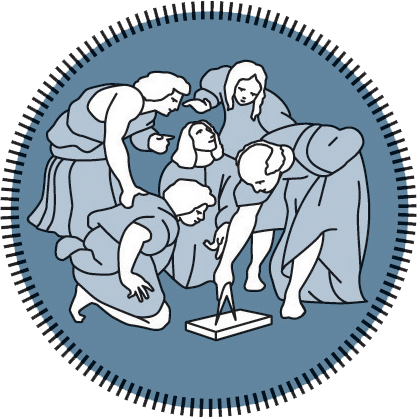
\includegraphics[scale=1.5]{Images/PolimiLogo.png}
	\end{center}

	\begin{center}
	 	{\Huge Politecnico di Milano}\\
	 	\vspace{5mm}
		{\Large A.A 2016-2017} 
		\vspace{5mm}\\
		{\huge Requirements Analysis and Specifications Document}   
		\vspace{5mm}\\
		{\large Version 1.0}  
    \end{center}
     
    \begin{center}
		\noindent\rule{8cm}{0.8pt}
		 \vspace{5mm}\\
 	 	 
\includegraphics[scale=1]{Images/logoPowerEnjoy2.png}\\
		\noindent\rule{8cm}{0.8pt}
	\end{center}
	 	\vspace{5mm}
	 		
	\begin{center}
	 	{\Large Instructor : Prof. Di Nitto}
	 	 \vspace{5mm}\\	 
	 	{\Large Authors:}\\
	 	{\Large Amico Simone}\\
	 	{\Large Chianella Claudia Beatrice}\\
	 	{\Large Giovanakis Yannick}
	\end{center}
	 
	\newpage
	
	%------------------
	%  CONTENTS TABLE
	%------------------
	
	\tableofcontents{}
	 
	\newpage
	 
	%-----------------
	%  1.INTRODUCTION
	%-----------------
	\section{\Large Introduction}
	 
	 %----------------
	 % 1.1 PURPOSE
	 %----------------
	 \subsection{Purpose}
		The aim of this document	is to give an overview of the requirements and 			
		specifications of the system to be developed. 
		The goal of the document is to describe in detail all functional and non-functional 
		requirements of the system, analyzing the needs of the customer and explaining common 
		use case scenarios.
		It will set a baseline for project planning and cost estimation, giving a detailed 
		insight to all stakeholders which include the PowerEnjoy Board , Investors and finally
	    engineers (present and future) involved  in development, testing and maintenance.
		
	 %----------------
	 % 1.2 SYSTEM
	 %----------------
	 \subsection{System}
	 	The to be developed software system provides a complete support to the new PowerEnjoy 	
	 	car-sharing service. It will allow users to register ,log-in and use the car sharing 
	 	service within the limits imposed by the below specifications.
	 
	
	 %----------------
	 % 1.3 SCOPE
	 %----------------
	 \subsection{\label{scope:1}Scope}
		The new PowerEnjoy software system will allow visitors to register and retrieve all 
		necessary information of common domain ( ToS , contact information...). \\Once the 
		visitor has successfully registered into the system and his/her driving license has been 
		approved, he/she will be provided with a unique username-password combination. This 
		enables a user to log into the system at any time , from any mobile device. \\Once 
		logged in, the user can search within a certain distance for vehicles based on his/her 
		current location or based on an input address. 
		Eventually the user chooses to reserve an available vehicle, which can be picked-up 
		within a time span of one hour.\\ 
		If the user doesn't pick-up the car within the one hour availability limit, then the 
		system will tag the vehicle as available and charge the user a fee of 1 Euro. \\
		If the user reach the car within the limit,he/she must be able to  interact with 
		the system in order to unlock the vehicle and grant the user access to the car.
		As soon as the engine ignites,the system starts charging the user for a given amount of 
		money per minute. The current charge will be notified through a display inside the car.	
		\\
		The system stops charging the user as soon as the car is parked in a safe area and the 
		user exits the car. At this point the system will automatically lock the car.
		If the user stops in a non-safe area he/she won't be granted to end the transaction 	
		and will be charged until  he/she parks in a safe area.
		The set of safe area parking spots is defined inside the system and must be available 	
		all the time to the user's knowledge through the on-board display.
		\newline
		In addition to the functionality above, the system should incentivize the virtuous 
		behaviours of the users with some bonuses:

	\begin{itemize}
		\item If the user shares a ride with at least two other passengers , the system will 
			  detect them and will apply a discount of 10\% the last ride.
		\item If the user parks the car in a safe area and the battery charge level is more 
			  than 50\% , the system will apply a discount of 20\% on the last ride.
		\item If the user parks the car in a safe area provided with a PowerEnjoy charging 
			  station and takes care of the recharing ,the system will apply a discount of 30
			  \% on the last ride.
		\item If the user parks the car in a safe area with a battery charge level less than 	
			  20\% or the distance to the next power grid is greater than 3 KM, the system 
			  will add a fee of 30\% of the last ride to compensate for the cost required to 
			  recharge the car on-site.
		\item If the user enables money saving option,he/ she can input the final destination 	
			  and the system provides information about the station where to leave the car to 
			  get a discount. This station is determined to ensure a uniform distribution of 
			  the cars in the city and depends both on the destination of the user and on the 
			  availability of power plugs at the selected station.
	\end{itemize}
	
	%--------------
	% 1.3.1 GOALS
	%--------------
	\subsubsection{Goals}
		The PowerEnjoy software system needs to be:
	\begin{itemize}
		\item \textbf{[G1] : Practical}\\It wants to give the users a better connectivity among 
					 places in the participant cities that common public transport often can't 
					 offer.
		\item \textbf{[G2] : Convenient}\\The service needs to be convenient: it's less 
					 expensive than taking a taxi. It's an eco-friendly solution : car-sharing 
					 reduces the number of vehicles circulating in the cities and doesn't 
					 pollute thanks to electric engines.
		\item \textbf{[G3] : User friendly}\\ The system needs to be as user friendly as 
				     possible in order to be used easily by everyone through their own 
				     intuitive knowledge. 
		\item \textbf{[G4] : Fast}\\ The system needs to be fast and responsive even during 
					 high peaks of activity.
		\item \textbf{[G5] : Available}\\ The system needs to be available at every time and on 
					 the largest possible number of devices (mobile and not) with an internet 
					 connection.
	\end{itemize}
	
	%-------------------
	% 1.3.2 APPLICATIONS
	%-------------------
	
	\subsubsection{Applications}
		To achieve the above mentioned goals the following software tools need to be developed:
	
	\begin{itemize}
		\item \textbf{Mobile Application}: to be developed for all major operating systems 
					 (iOS, Android , Windows Phone). The mobile software must allow the user 
					 to perform all the tasks in the \hyperref[scope:1]{\textit{Scope section 
					 (1.3)}}.
		\item \textbf{Web Application}: must be compatible with all major browser applications (Chrome, Firefox, Safari, Edge, Opera). 
					 The user must be allowed to perform all tasks in  the \hyperref[scope:1]
					 {\textit{Scope section (1.3)}}.
		\item \textbf{ On board car application}: this application needs to handle user 
					 interaction such as displaying general car information (charge, fee, tire 
					 pressure...), letting the user validate his/her identity through a pin 
					 code and report about the status of the vehicle. 
					 Furthermore it must control if the vehicle is parked in a safe area.
		\item \textbf{ Back-End Application}: this application handles all search and 
					 reservation requests, payment transactions and car communications. It is
					 also an essential tool for customer support operators.
	\end{itemize}
		
	%-----------------------
	% 1.4 REFERNCE DOCUMENTS
	%-----------------------
	\subsection{Reference Documents}
	\begin{itemize}
		\item IEEE Std 830-1998: “IEEE Recommended Practice for Software Requirements 	
			  Specifications”
	 	\item Project description: “Assignments AA 2016-2017.pdf”
	 	\item Alloy Language Reference : \url{http://alloy.mit.edu/alloy/documentation/book-	
	 		  chapters/alloy-language-reference.pdf}
	 	\item UML Language Reference : \url{https://www.utdallas.edu/˜chung/Fujitsu/UML_2.0/
	 		  Rumbaugh--UML_2.0_Reference_CD.pdf}
	\end{itemize}
	
	%-----------------------
	% 1.5 GLOASSARY
	%-----------------------
	 
	\subsection{\label{actors:3}Glossary}
	 
	 %--------------
	 % 1.5.1 ACTORS
	 %--------------
	 \subsubsection{Actors}
     \begin{itemize}
 	 	\item \textit{Visitor}: a visitor is defined as a person who is not logged into the 	
 	 				 system.
  		\item \textit{Registered User}: is defined as customer who is  logged into the system.
  		
  		\item \textit{Car}: is defined as the mean of transport to be used by a registered 
  					 user.
  		\item \textit{Support operator}: The support operator is an employee who is trained and 
  					 has a full grasp of the different software application.
	\end{itemize}
	
	 %------------------------
	 % 1.5.2 OTHER DEFINITIONS
	 %------------------------
	 \subsubsection{Other definitions}
	 \begin{itemize}
		\item \textit{Valid Payment}: as payment we accept only Credit Cards (Visa, MasterCard 
			  and American Express).\\The payment method must be valid : the card must not be 
			  expired nor blocked. The validity will be checked immediately during registration 
			  phase.
		\item \textit{Valid Drivers License}: the user must be provide a valid european drivers 
			  license. The license must be valid: it must not be expired or suspended. The 
			  validity will be checked immediately during registration phase. 
		\item \textit{Safe Area} : a safe area is any part of the city where the user is 
			  allowed to park. Safe areas are pre-defined and installed into the cars' on board 
			  systems. If a user parks the car in an area which is \textit{not} safe , he/she 
			  will not be able to end the ride and will be charged until he/she parks in a safe 
			  area.
		\item \textit{Money Saving Option}: when a user starts a ride he/she can enable this 
			  mode on the onboard display: he/ she can input the final destination and the 
			  system provides information about the station where to leave the car to get a 
			  discount.
		\item \textit{Reserved Car}:  is a vehicle currently used by a user. Reserved cars are 
			  not visible as results of a search query.
		\item \textit{Time left to unlock}: as soon as a user reserves a car, he/she has one 
			  hour to unlock it. The time left is displayed on top of the user's mobile/web 
			  application.
		\item \textit{Charging Station}: all PowerEnjoy's cars are provided with an electric 
			  engine. A charging station is a location where the user can park and recharge the 
			  car. All charging stations are listed in the on- board system.
		\item \textit{Battery level} : the current state of the battery charge is indicated by 
			  the battery level.
		\item \textit{Passenger} : is a person ( not necessarily registred ) who shares a ride 
			  with a registred driver. A passenger cannot drive but his presence will be 	
			  detected by the system. 
		\item \textit{On-board application}: is the software installed on every car. The user 
			  can interact with it through a touch screen display.
		\item \textit{Mobile application}: is the downloadable software that can be installed 
			  on major mobile devices.
		\item \textit{Web application}: is the online software that is accessible through all 			 	  common web browsers.
		\item \textit{Back-End application}: is the part of the system that manages queries 
			  ,data and user-system interaction.
		\item \textit{Ride}: a ride is a time span starting from the moment the user turns the 
			  car on and ends when the user parks it in a safe area after the car has 
			  automatically locked the doors.
		\item \textit{Payment History} : a chronological list of all payments and rides made by 
			  a given user.
		\item \textit{Available car} : a car that is not reserved or charging. These cars are 
			  shown as result of search queries and can be reserved by users.
	\end{itemize}		
	
	
	%-------------------
	%	1.6 DOC OVERVIEW
	%-------------------
	
	\subsection{Document overview}
	\begin{enumerate}
		\item \textbf{Introduction}: this section gives a general 	description of the 
			  software and its characteristics 
		\item \textbf{Overall description}: this section gives a detailed overview of the 
			  document focusing on domain assumptions, requirements (functional and not) and 
			  the characteristics of different types of interacting users.
		\item \textbf{Specifications}: this section gives a deep insight about the system's 
			  main functionality, analyzing scenarios with their relative use-cases and 
			  includes an extensive alloy model. Event flows are model using sequence and state 
			  diagrams.
	\end{enumerate}	
	\newpage
	

  %-----------------------
  %	2. DOCUMENT OVERVIEW
  %----------------------- 
  \section{\Large Overall Description}
  	The overview section highlights all the main functionality and constraints of the 	
	PowerEnjoy software.  
	
	%----------------------
	% 2.1 SOFTWARE OVERVIEW
	%----------------------
	
	\subsection{Software overview}
	 \begin{center}
 	 	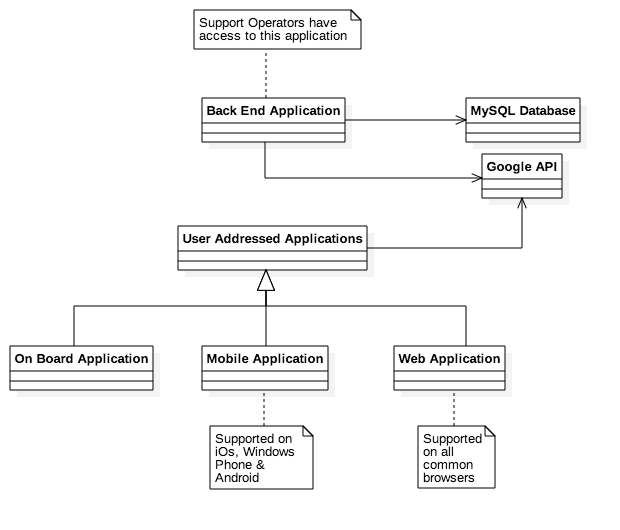
\includegraphics[width=0.9\textwidth ,height=0.9\textwidth ,center]
 	 				    {Images/SoftwareDistribution.png}
	 \end{center}
	
	
	
	%-------------------------
	% 2.2 USER CHARACTERISTICS
	%------------------------- 
	 
	 	
	\subsection{User characteristics}
		Specifies the characteristics of the different actors mentioned in \hyperref[actors:3]	
		{\textit{Actors section (1.5.1)}} 
	\begin{itemize}
		\item \textbf{Visitor}: A visitor can see only the log-in page with a registration form 
	     	  and some common information ,such as the company's customer office contact 
	     	  information and terms of service. There are no constraints about visitors : every 
	     	  person can access the main site and try to register.
		\item \textbf{User}: a want-to-be user must match the following requirements:
		\begin{itemize}
				\item the user has to be \textbf{at least 18} years old
				\item the user must have a \textbf{valid} driving license \footnote{\label{note1} For 
			    more check out the \hyperref[actors:3]{\textit{Glossary}}}
				\item the user must enter a \textbf{valid} payment method 
	    \end{itemize}
		\item \textbf{Car}: is property of the PowerEnjoy Company. A car must be able to 		
				communicate to with the system all the time. If a car is available (i.e 		
				currently not reserved by a registered user) then its current location must be 
				stored in the system so to be shown on all users' devices. As soon as the 
				engine ignition starts , the car's system must time the vehicle's usage in 
				order to charge the user the right amount of money. Once the user has parked 
				the car inside a safe area and has exited, the car informs the system about 
				the fee to charge ,locks the doors automatically and finally informs the 
				system that it is available again.
		\item \textbf{Support Operator}: his job is to offer costumer support concerning 
				software issues and help out in case of emergency.\\ Contrary to a user, he 
				has access to the back-end software which enables him to overview the system 
				status.
	\end{itemize}
	
	%-------------------------
	%	2.3 DOMAIN ASSUMPTIONS
	%-------------------------
	
	\subsection{Domain assumptions}
		
		%-----------------------------------
		%	2.3.1 GENERAL DOMAIN ASSUMPTIONS
		%-----------------------------------
		
		\subsubsection{General Domain Assumptions}
			We hold the assumption that the system will be deployed in large metropolitan 
			cities with a maximum of 3M inhabitants.\\
			We assume that the mean highest peak of activity is around dinner time on Fridays 
			and Saturdays. We assume that during the peak the system will be used by around 50k 
			people , 80\% of which gain access to the system through the Mobile Application, 
			while the remaining 20\% through the Web Application.\\
			We assume that the the fleet of vehicles will be proportional to the number of 
			inhabitants, reaching a peek of 300 vehicles in the biggest area.\\
			
		%---------------------------------
		%	2.3.2 USER ASSUMPTIONS
		%---------------------------------		
		\subsubsection{User Assumptions}
			We assume that all users are provided with an enabled internet connection equipped 	
			with GPS tracking which is the only way to search, reserve and unlock a car.
			We assume that all active users carry their driving license with them and drive 
			following the traffic code\footnote{\url {http://www.mit.gov.it/mit/site.php?
			p=normativa&o=vd&id=1&id_cat=&id_dett=0}}.

		%-------------------------------
		%	2.3.3 VEHCILE ASSUMOPTIONS
		%-------------------------------
		\subsubsection{Vehicle Assumptions}
		* chiedere se e' bisogna inserire assunsiozioni sulla carica delle macchine etc...*		
	
	
	%----------------------
	%	2.4 CONSTRAINTS
	%----------------------		
	\subsection{Constraints}
	
		%-----------------------------
		%	2.4.1 SOFTWARE LIMITATIONS
		%-----------------------------
		\subsubsection{Software Limitations}
			The Mobile and Web Application can not exceed 50MB of RAM usage.\\
			The On-Board application can not exceed 75MB of RAM usage.\\
			The Back-End application cannot exceed 100GB of RAM usage.
		\newpage
		%-----------------------------
		%	2.4.2 HARDWARE LIMITATIONS
		%-----------------------------
		\subsubsection{Hardware limitations}
		The Mobile Application must be available for the following mobile operating systems:
		\begin{itemize}
			\item iOS version 7.0 or higher.
			\item Android version 4.0 or higher.
			\item Windows Phone 8 or higher.
		\end{itemize}
		The applications must interface with Google Maps API \footnote{\url{https://	
		developers.google.com/maps/documentation/javascript/}} and follow the design guidelines 
		provided by each platform \footnote{\url{https://developer.android.com/design/
		index.html}} \footnote{\url{https://developer.apple.com/design/}}.\\
		\newline
		The Web Application must be developed in order to be correctly used by the following 
		web browsers \footnote{\url{http://www.w3schools.com/browsers/default.asp}}:
		\begin{itemize}
			\item Mozilla Firefox
			\item Google Chrome
			\item Safari
			\item Microsoft Edge
			\item Opera
		\end{itemize}
		The on-board software system must be equipped with a GPS Module and interface Google 
		Maps API. The following safety regulations must be followed:
		\begin{itemize}
			\item \textbf{Night mode}: an automatic night mode must be implemented. This will 
				  avoid that drivers get blinded by excessive brightness of the display.
			\item \textbf{Safe - area parking recognition}: the system must recognize whether 
				  the vehicle is parked in a safe-area or not.
			\item \textbf{Additional passenger recognition}: the system must recognize 
				  passenger. This feature is crucial for bonus credit distribution to the 	
				  driver.
		\end{itemize}
	
		%----------------------
		%	2.4.3 CONCURRENCY
		%----------------------
		\subsubsection{Concurrency}
		The back-end application must be able to handle correctly multiple user requests 
		without creating conflicts : if two users desire two reserve the same car 
		simultaneously ,only one can be granted a reservation.
		
		%----------------------------
		%	2.4.4 REGULATORY POLICIES
		%----------------------------
		\subsubsection{Regulatory Policies}
		\begin{itemize}
			\item \textbf{Privacy Policy}: Data should be collected and stored following the 
			  privacy policy guidelines provided by Mozilla Foundation \url{https://
			  developer.mozilla.org/en-US/Marketplace/Publishing Policies_and_Guidelines/
			  Privacy_policies}
			\item Network connections must be encrypted.
			\item Data storage on PowerEnjoy databases must be encrypted
		\end{itemize}
		
	  %------------------------------
	  % 2.5 FUNCTIONAL REQUIREMENTS
	  %------------------------------

	  \subsection{Functional Requirements}
	  \textbf{1.Mobile and Web Application}
	  \begin{itemize}
	 		\item{\textbf{[R1.1]}}: Allow a guest to register entering all relevant personal 
	 			 data and a valid driving license whose validity will be check on the spot
	 		\item{\textbf{[R1.2]}}: Allow a registered user to log-in
	 		\item{\textbf{[R1.3]}}: Allow a registered user to update his personal information
	 		\item{\textbf{[R1.4]}}: Allow a registered user to search for an available vehicle 
	 			 given his position within a selected distance
	 		\item{\textbf{[R1.5]}}: Allow a registered user to search for an available vehicle 	
	 			 given an input position within a selected distance
	  		\item{\textbf{[R1.6]}}: Allow a registered user to reserve a selected vehicle.
	 		\item{\textbf{[R1.7]}}: Allow a registered user to check his payment history
	 		\item{\textbf{[R1.8]}}: Allow a registered user to recover his account log-in 	
	 			 information in a secure way
	 		\item{\textbf{[R1.9]}}: Allow a registered user to search for an available vehicle 	
	 			 given an input position.
	 		\item{\textbf{[R1.10]}}: Allow a registered user to unlock \emph{his/her} reserved 	
	 			 car if the user is nearby.
	 		\item{\textbf{[R1.11]}}: **Chiedere per cancellazione prenotazioni**
	 	\end{itemize}

		\textbf{2.On-Board Application}
		\begin{itemize}
	 		\item{\textbf{[R2.1]}}: Allow a registered user to correctly identify himself/
	 			 herself 	by entering a user specific pin-code
 	 		\item{\textbf{[R2.2]}}: Enable a registered user to keep track of the distance 
 	 			 covered, time spent using the car ,the current owed fee and the remaining 	
 	 			 battery charge.
 	 	\end{itemize}
 	 
 	 	\textbf{3.Back-End Application}
		\begin{itemize}
	 		\item{\textbf{[R3.1]}}: .
 	 	\end{itemize}
	
	  %-----------------------------
	  %  NON FUNCTIONAL REQUIREMENTS
	  %-----------------------------
	  \subsection{Non functional Requirements} 
	  	Some non functional requirements have been to be necessary in the to be developed 
	  	system in order to provider a correct operation flow and an optimized UX.
		\begin{itemize}
			\item \textit{User friendliness}: the Mobile/Web as well as the On-Board 
				  Application must be easily handled by the average web user with basic web 	
				  knowledge.
			\item \textit{Performance}: to supply a suitable service the system must be 
				  responsive even at peak activity times. To achieve this client-server 
				  transaction must be reduced to a minimum.
		 	\item \textit{Reliability}: the PowerEnjoy service must be active 24h/24h . 
		 		  Maintenance must be performed without compromising functionality. At all the 
		 		  time , a user must be able to be charged the owed fee.	
		 	\item \textit{Data integrity and availability}: 
	   		 	  Data have to be always available and accessible.Data availability can be 
	   		 	  achieved by duplicating data on back-up servers. For instance the use of 
	   		 	  RAID, mirroring and backup could present a valid solution.

		 	\item \textit{Maintainability}: the software should be implemented so as to be as 
		 		  modular as possible to allow future expansions and easy modifications\\
		 		  Google API are required but can be easily updated from time to time on all 
		 		  systems.
		 	\item \textit{Security}: user accounts are provided with two factor authentication 
		 		  with a code sent to the user's mobile phone to add a secure connection 
		 		  method to the system. Sensible user information are stored using a hashing 
		 		  mechanism .\\User data input should be filtered to avoid malicious 
		 		  modifications ( i.e SQL Injections). \\All connections should be encrypted 
		 		  and run on a secure HTTPS protocol with valid certificates that uses the 
		 		  secure TSL protocol to avoid Man in the Middle Attacks.
		\end{itemize}
		
	%--------------------------
	% 2.6 FUTURE IMPLEMENTATION
	%--------------------------
	\subsection{Future implementation}
		The system must be as scalable as possible: future implementations can require a 
		deployment in very large metropolitan cities that exceed by far the maximum amount of 
		planned users.\\ An important thing to keep in mind is that the nature of vehicles 
		could change in the distant future : not only cars , but also electric powered 
		motorcycles could be added to the PowerEnjoy vehicle fleet.This means that the on-
		board software should be as expandable as possible using for instance Hierarchy Design 
		Patterns in the vehicle type definition.
	 

	\newpage

 %-------------------------
 % 3. SPECIFIC REQUIREMENTS
 %-------------------------
 	\section{\Large Specific Requirements}
	
		%-------------------
		%	3.1 EX INTERFACE
		%-------------------
 		\FloatBarrier
		\subsection{External Interface Requirements}
 			This section is dedicated to illustrate the mockups of the user interfaces.

 		%-------------------
		%	3.1.1 MOBILE
		%-------------------
 		\subsubsection{Mobile Application}
		\begin{figure}
		 \vspace{-15cm}
		 \minipage{0.50\textwidth}
		 \centering	
		 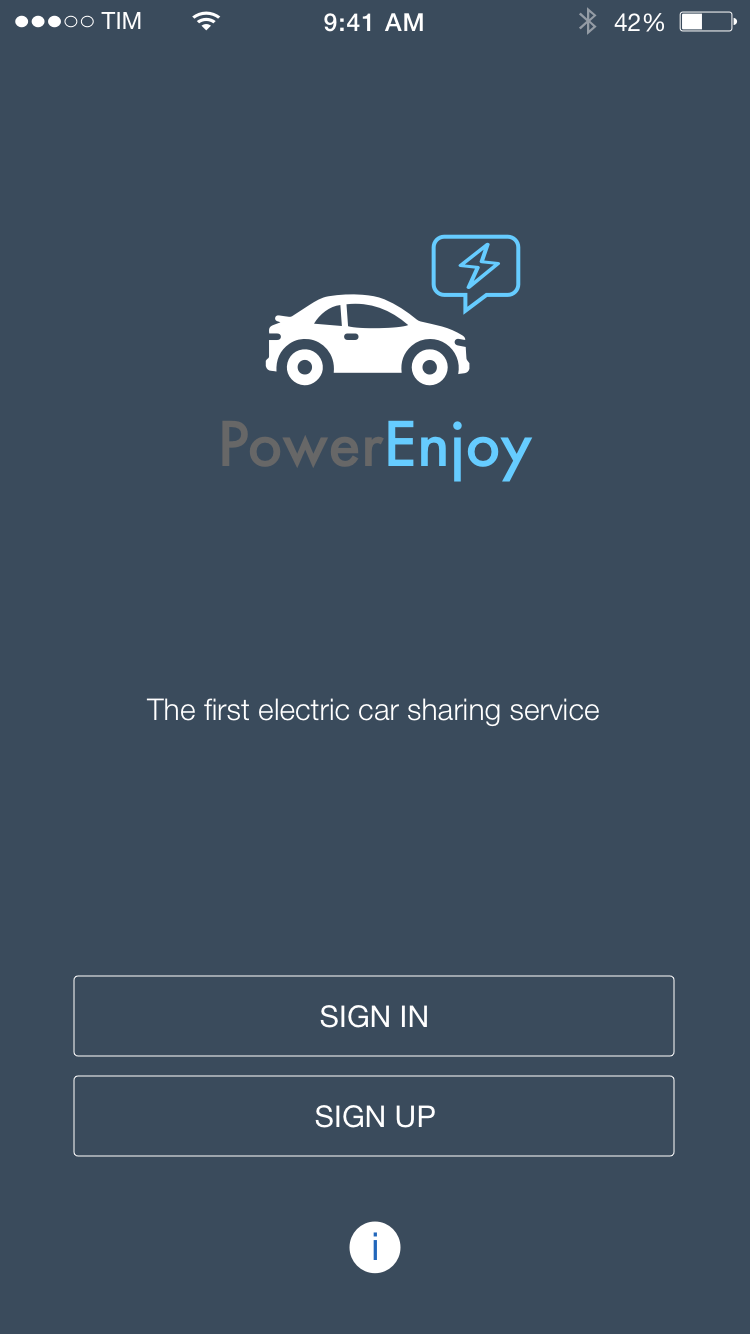
\includegraphics[scale=0.25]{Images/mobileApp/Home.png}
		 \caption{Confirm selection}
		 \endminipage
		 \minipage{0.50\textwidth}
		 \centering
 	 	  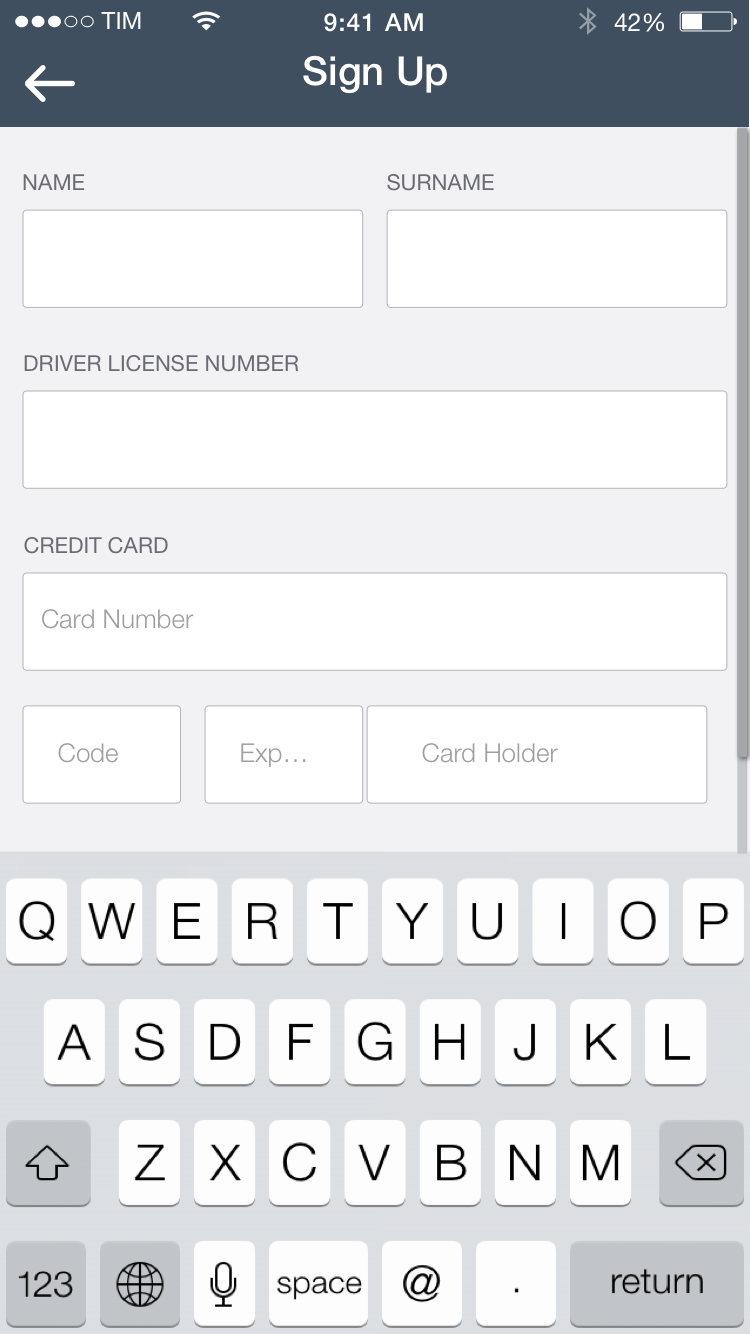
\includegraphics[scale=0.25]{Images/mobileApp/Register.png}
		  \caption{Time left to unlock}
		  \endminipage
 	 	\end{figure}
 	 	\clearpage
 	 	
 	 	\begin{figure}
		 \minipage{0.50\textwidth}
		 \centering	
		 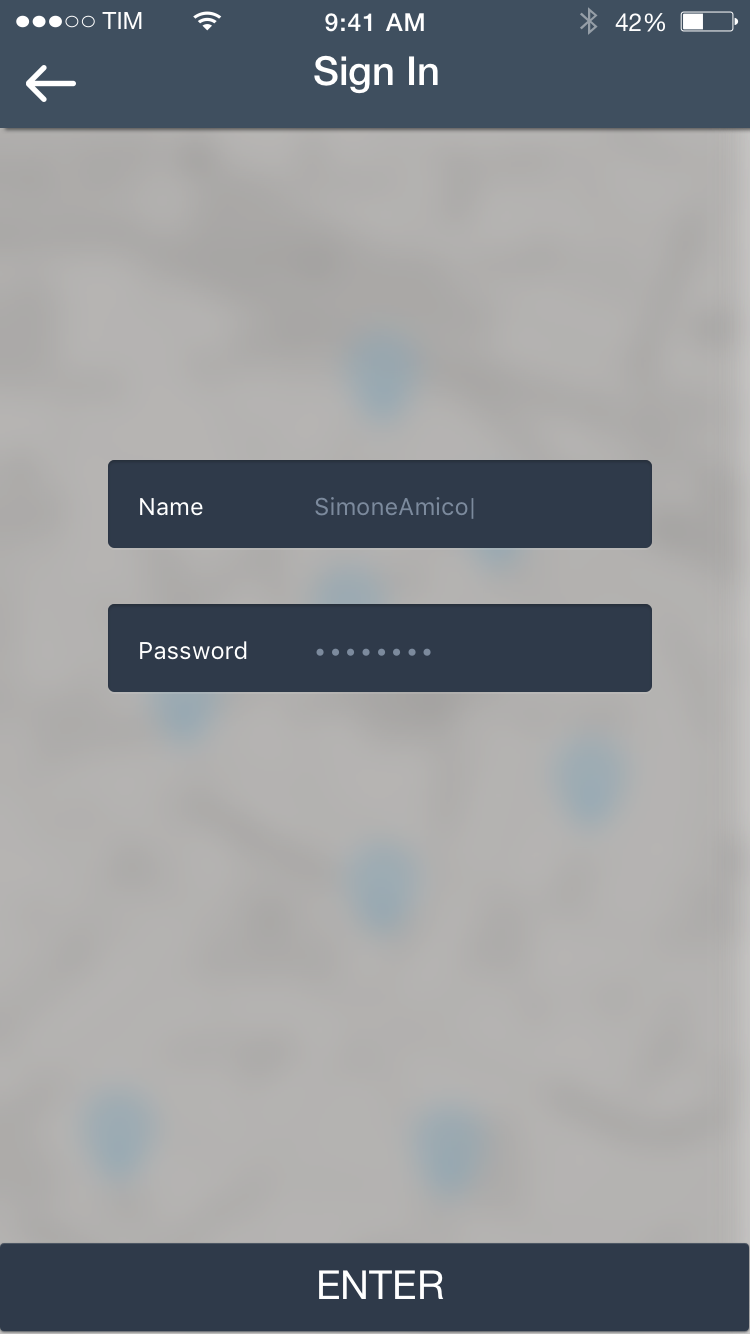
\includegraphics[scale=0.25]{Images/mobileApp/SignIn.png}
		 \caption{Sign In}
		 \endminipage
		 \minipage{0.50\textwidth}
		 \centering
 	 	  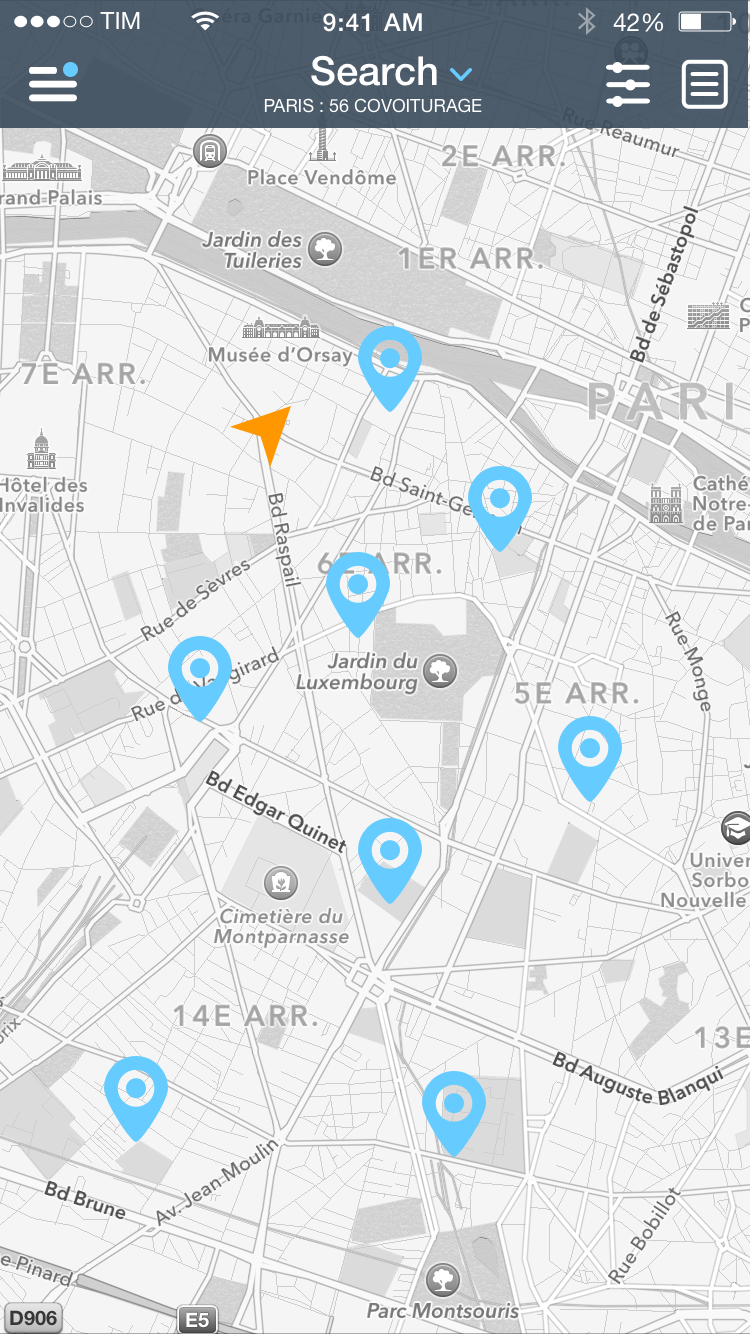
\includegraphics[scale=0.25]{Images/mobileApp/RicercaMappa.png}
		  \caption{Search}
		  \endminipage
 	 	\end{figure}
		\clearpage
		\begin{figure}
		 \minipage{0.50\textwidth}
		 \centering	
		 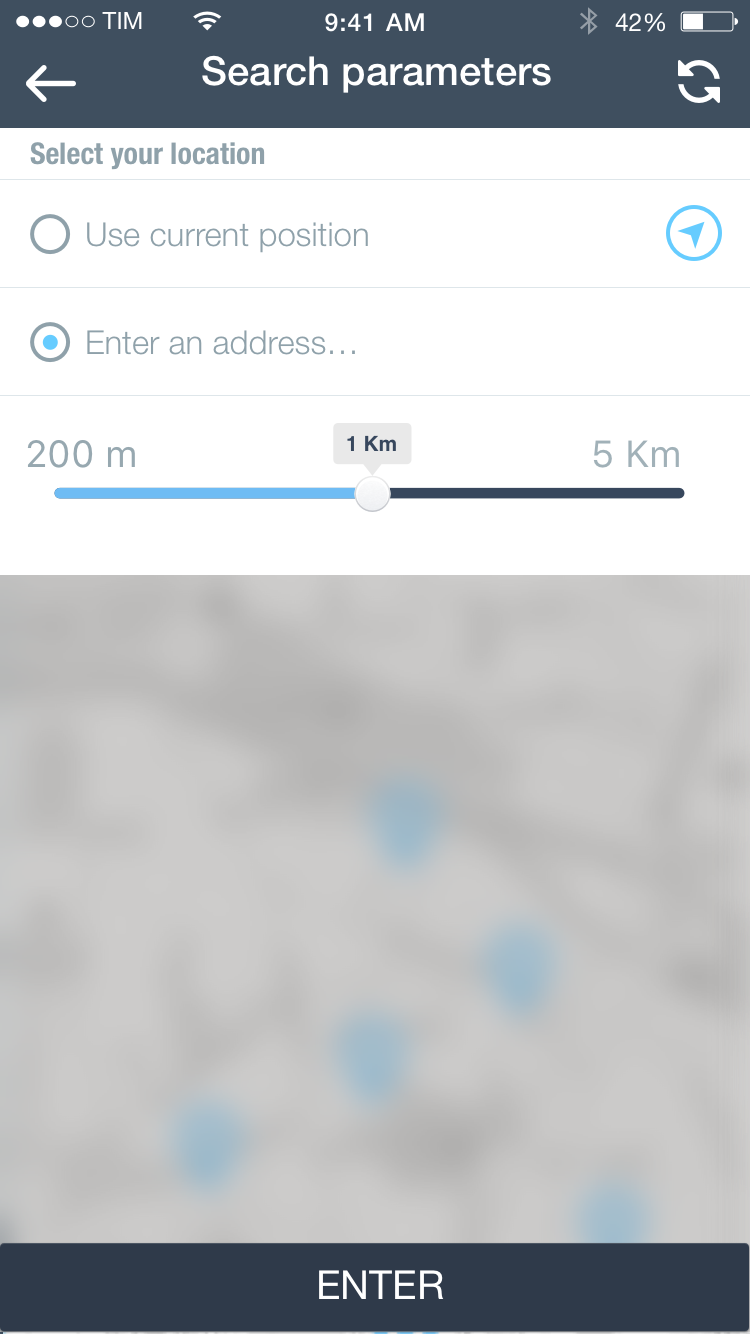
\includegraphics[scale=0.25]{Images/mobileApp/Param.png}
		 \caption{Address input}
		 \endminipage
		 \minipage{0.50\textwidth}
		 \centering
 	 	  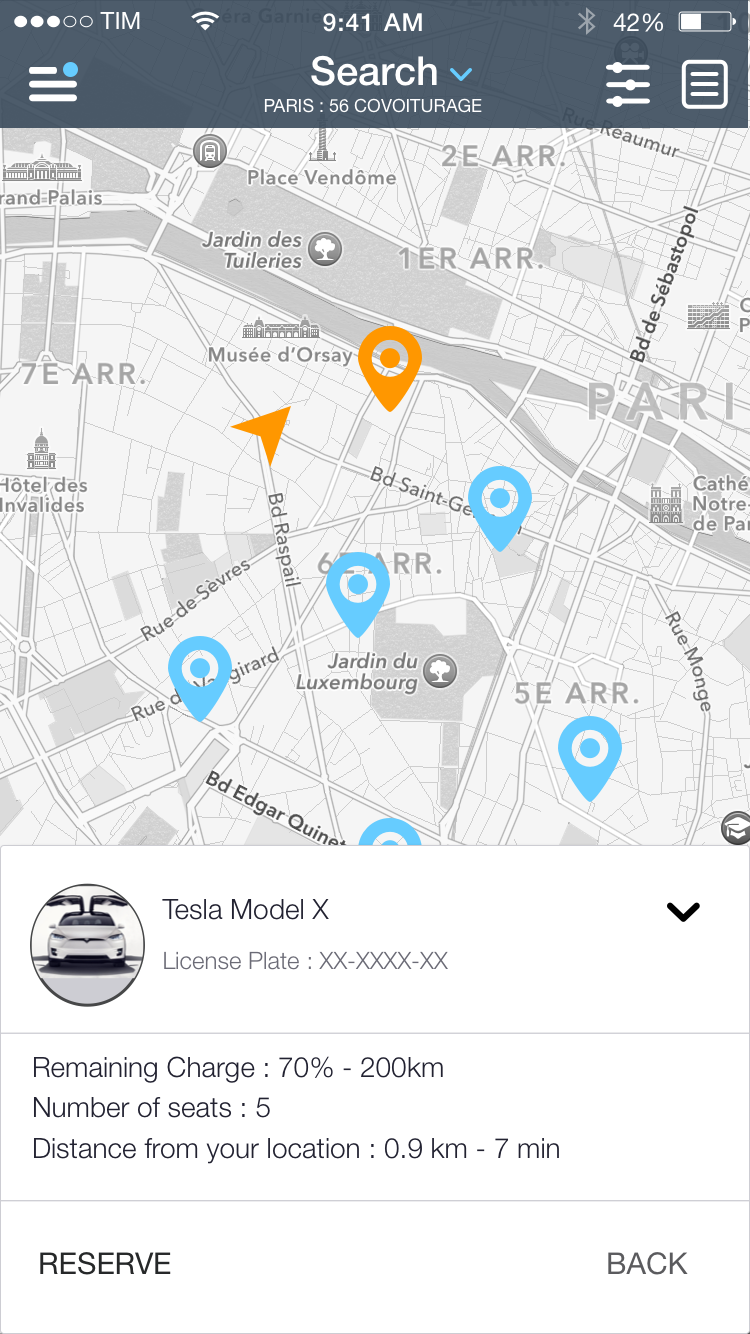
\includegraphics[scale=0.25]{Images/mobileApp/SelCar.png}
		  \caption{Car Selection}
		  \endminipage
 	 	\end{figure}
 	 	\clearpage
 	 	
 	 	\begin{figure}
		 \minipage{0.50\textwidth}
		 \centering	
		 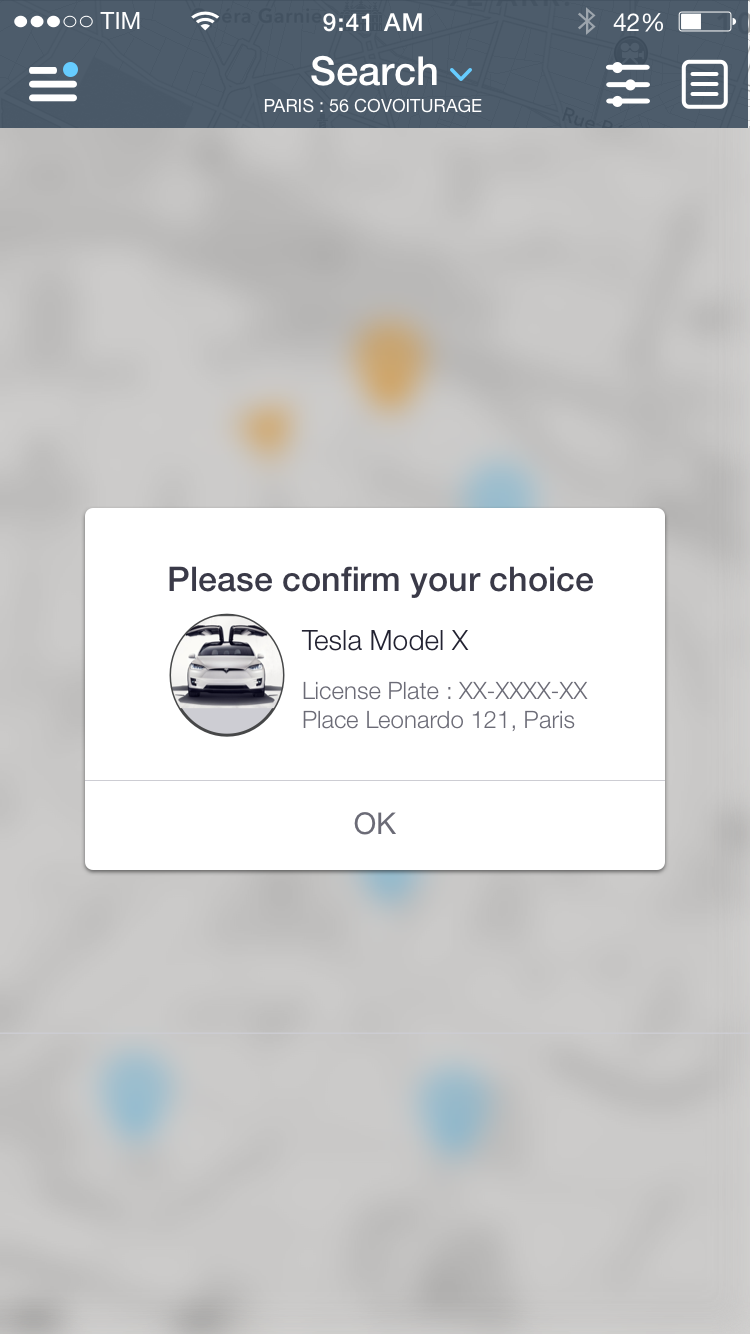
\includegraphics[scale=0.25]{Images/mobileApp/Conferma.png}
		 \caption{Confirm selection}
		 \endminipage
		 \minipage{0.50\textwidth}
		 \centering
 	 	  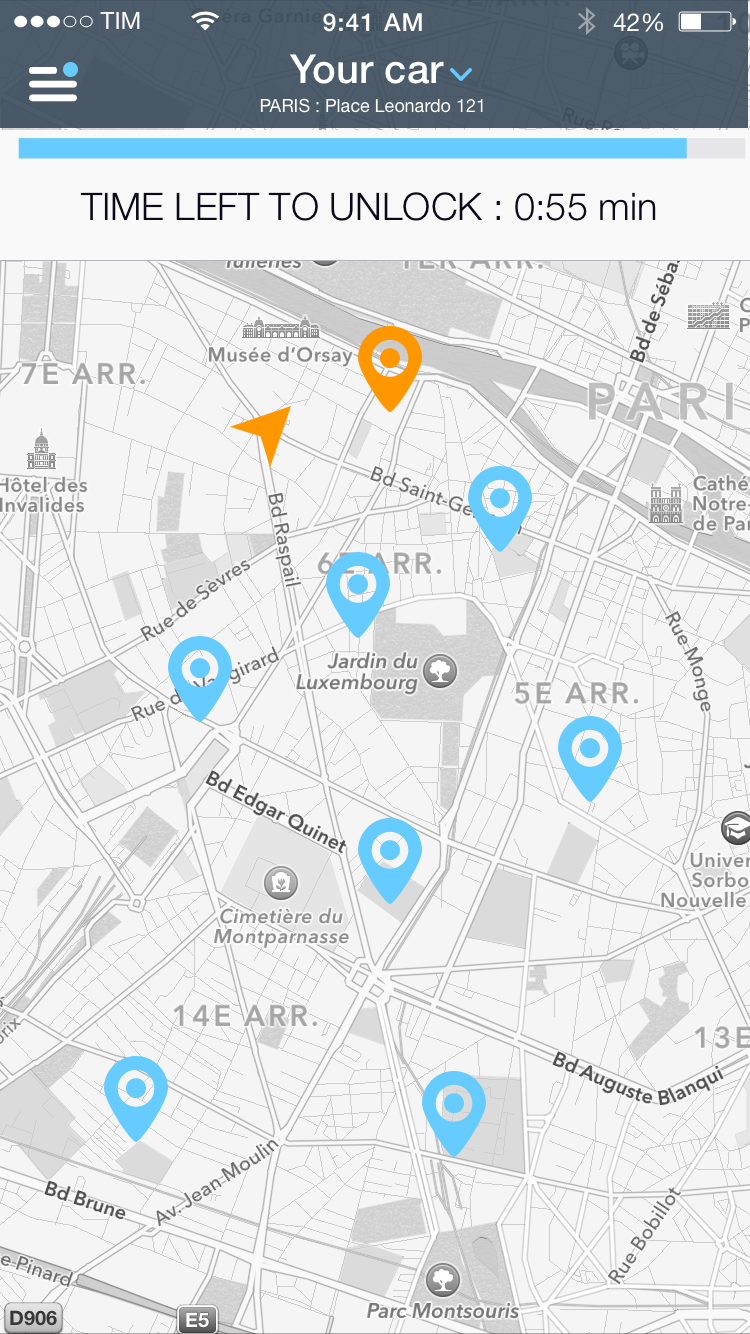
\includegraphics[scale=0.25]{Images/mobileApp/TimeLeft.png}
		  \caption{Time left to unlock}
		  \endminipage
 	 	\end{figure}
 	 	\clearpage
 	 	
 	 	\begin{figure}
		 \minipage{0.50\textwidth}
		 \centering	
		 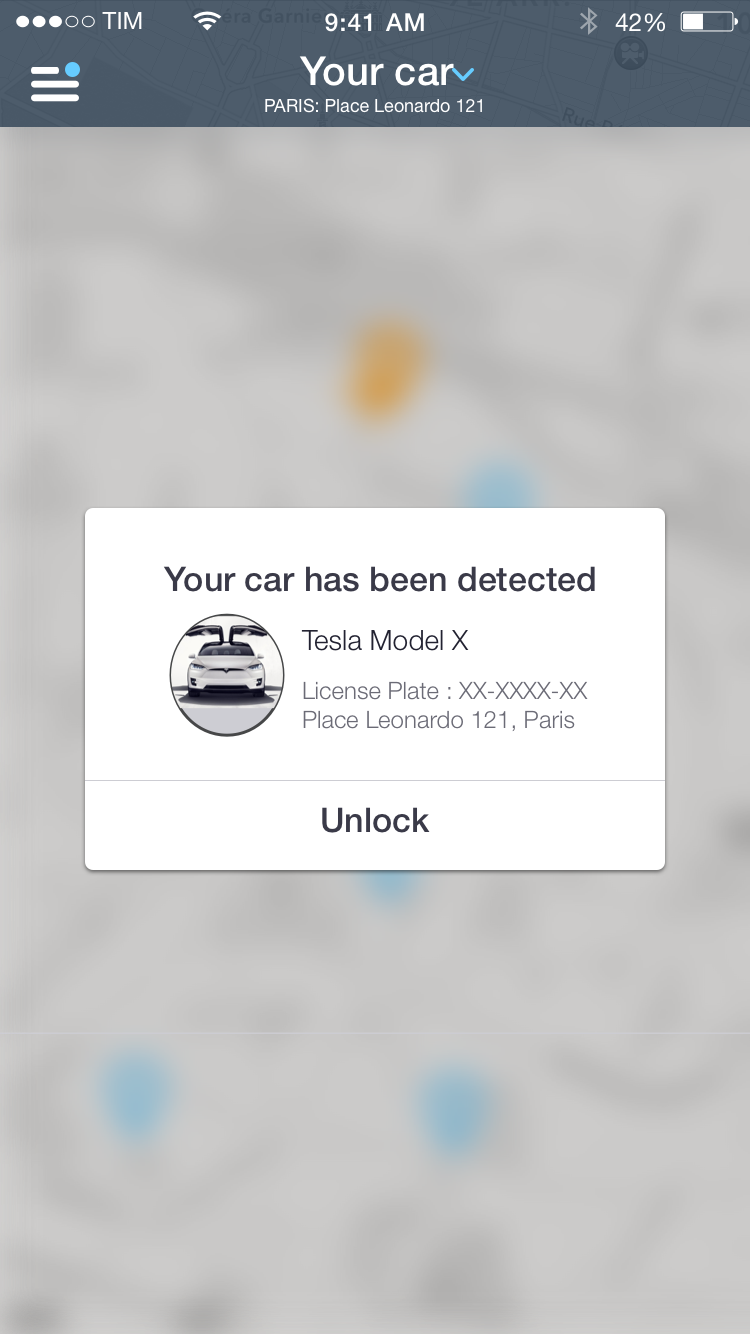
\includegraphics[scale=0.25]{Images/mobileApp/Sblocca.png}
		 \caption{Unlock car}
		 \endminipage
		 \minipage{0.50\textwidth}
		 \centering
 	 	  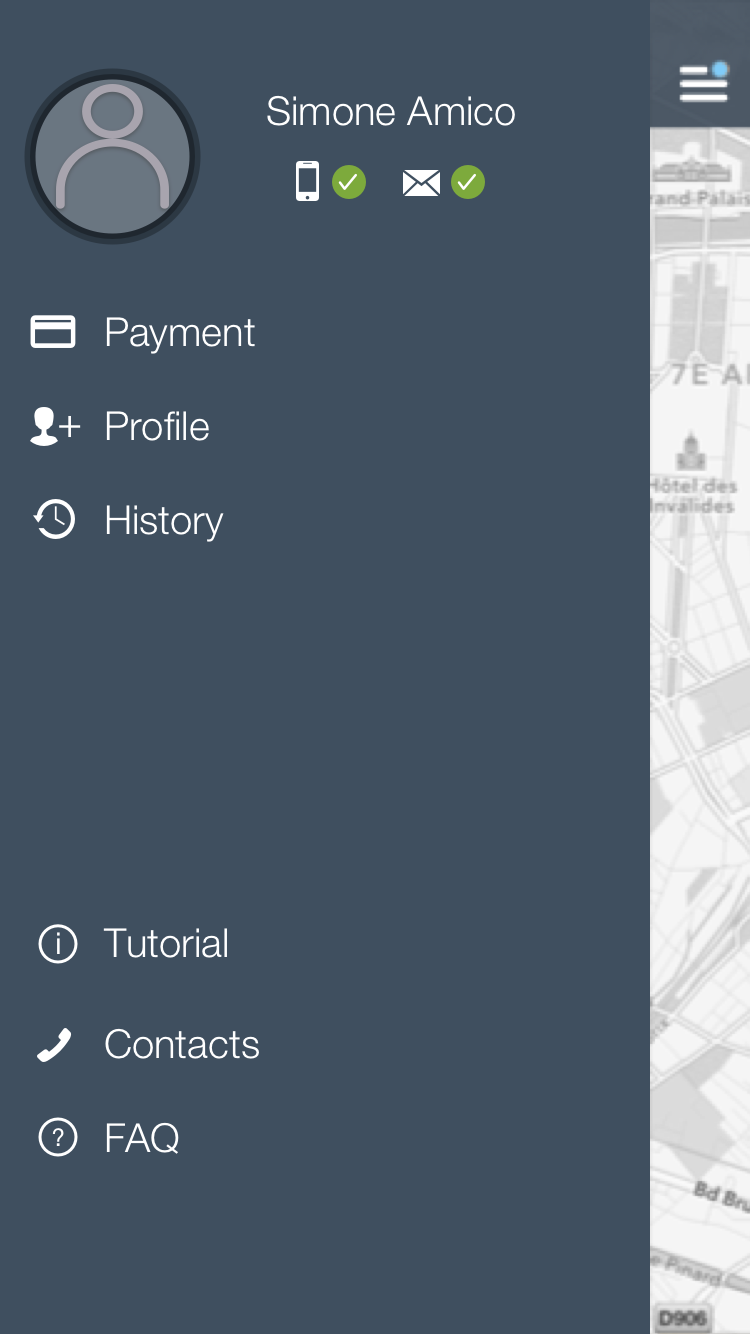
\includegraphics[scale=0.25]{Images/mobileApp/Menu.png}
		  \caption{Menu}
		  \endminipage
 	 	\end{figure}
 	 	\clearpage
 		%-------------------
		%	3.1.2 WEB 
		%-------------------	 
 	 	\FloatBarrier
 	 	\subsubsection{Web Application}
 	  	\begin{figure}
		\centering	
		\vspace{-14cm}		 
		 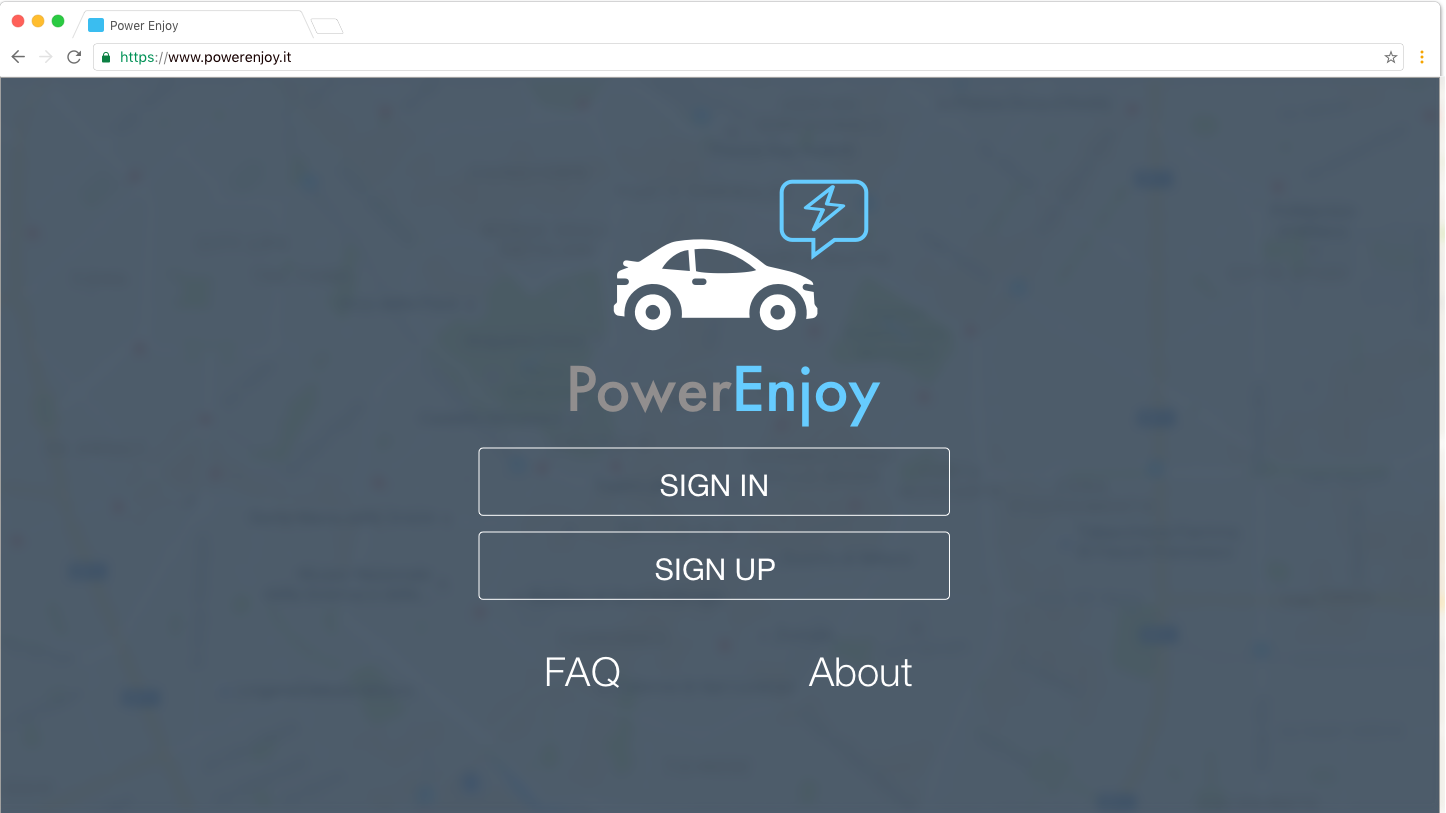
\includegraphics[scale=0.28]{Images/webApp/Homepage.png}
		 \caption{Homepage}
		 \centering
 	 	  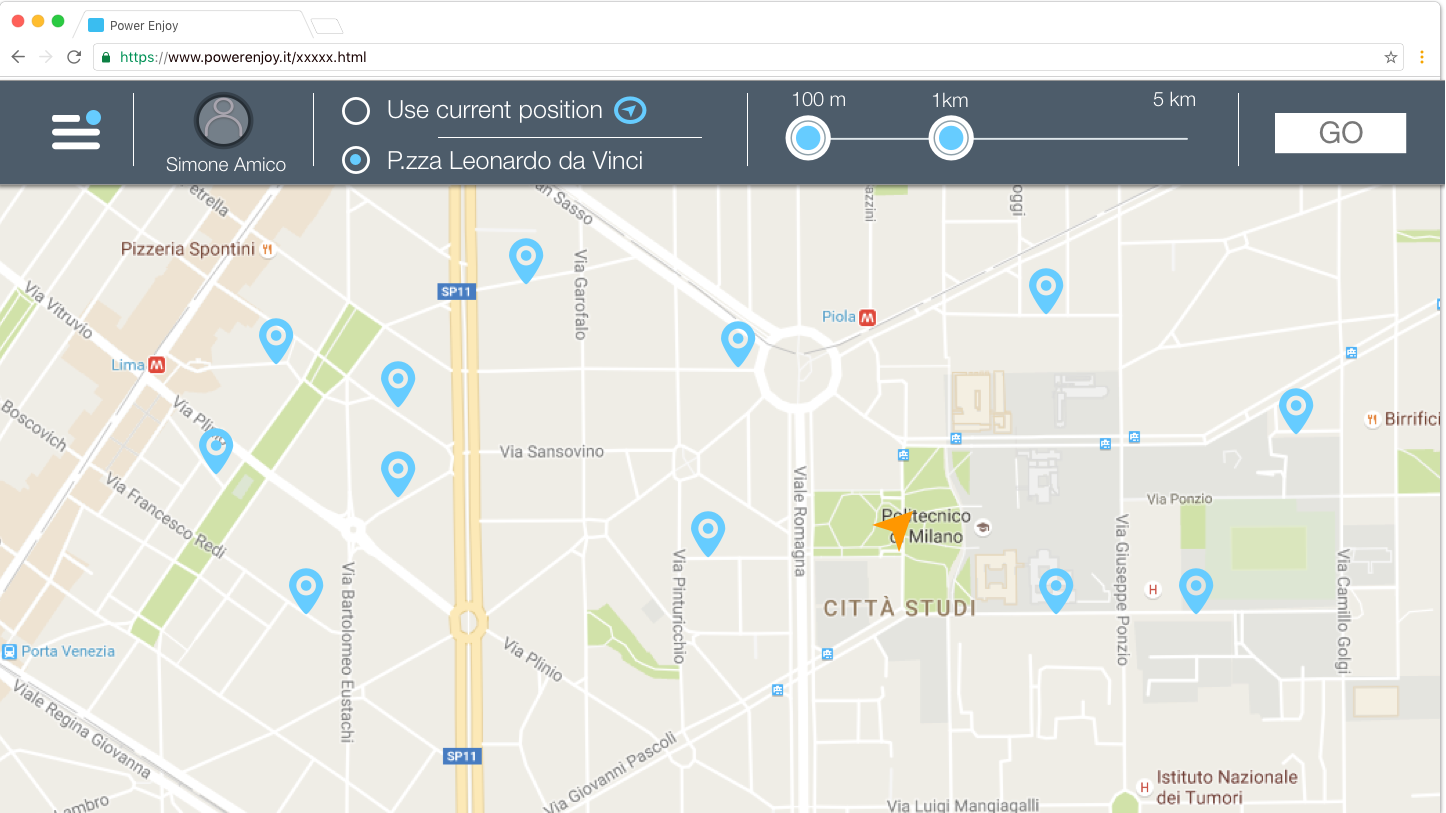
\includegraphics[scale=0.28]{Images/webApp/MainSearch.png}
		  \caption{Main page with map an car locations}
 	 	\end{figure}
 	 	\clearpage
 	 	
 	 	\begin{figure}
 	 	 \centering
 	 	 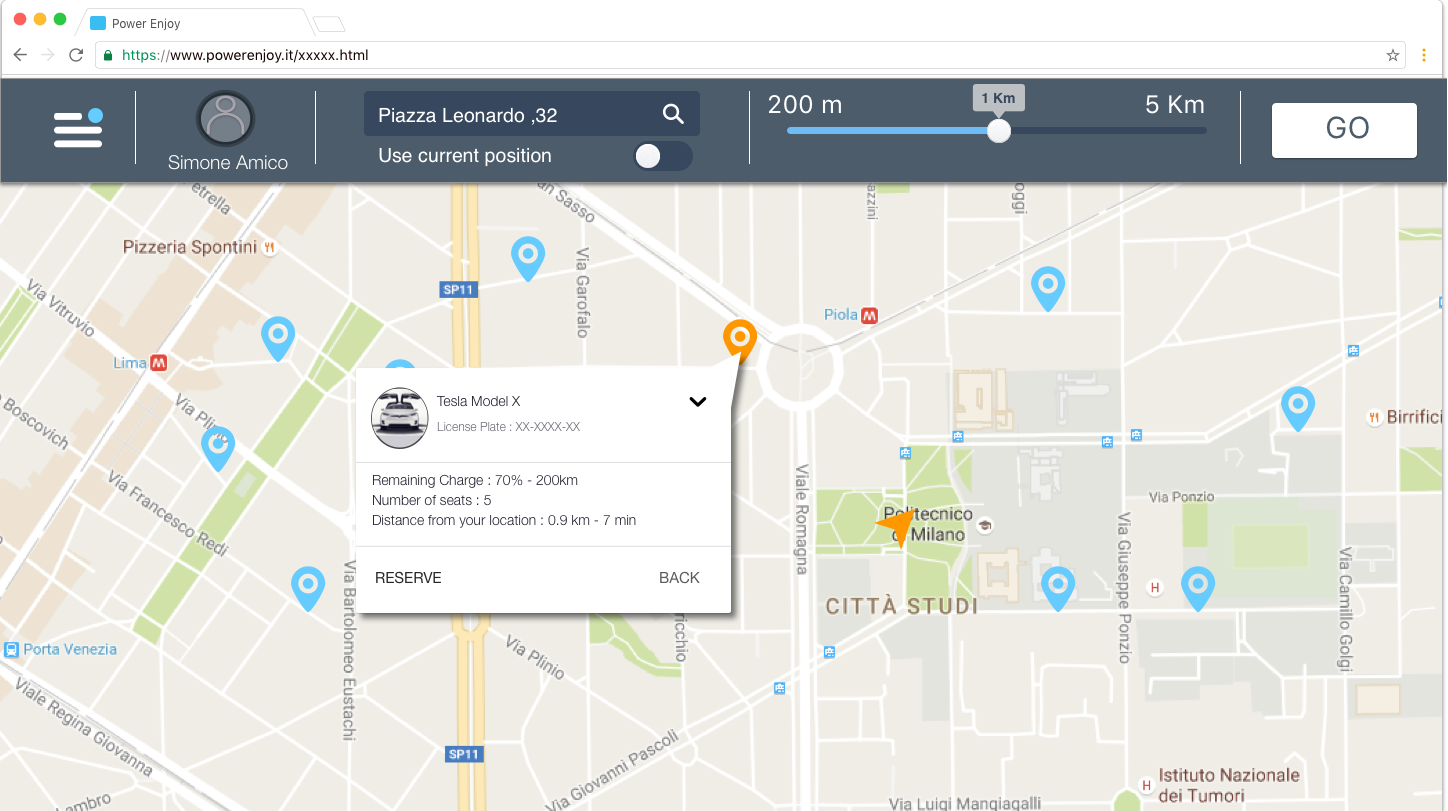
\includegraphics[scale=0.28]{Images/webApp/MainSearchCar.png}
		 \caption{Main page with car selection}
 	 	 \centering
 	 	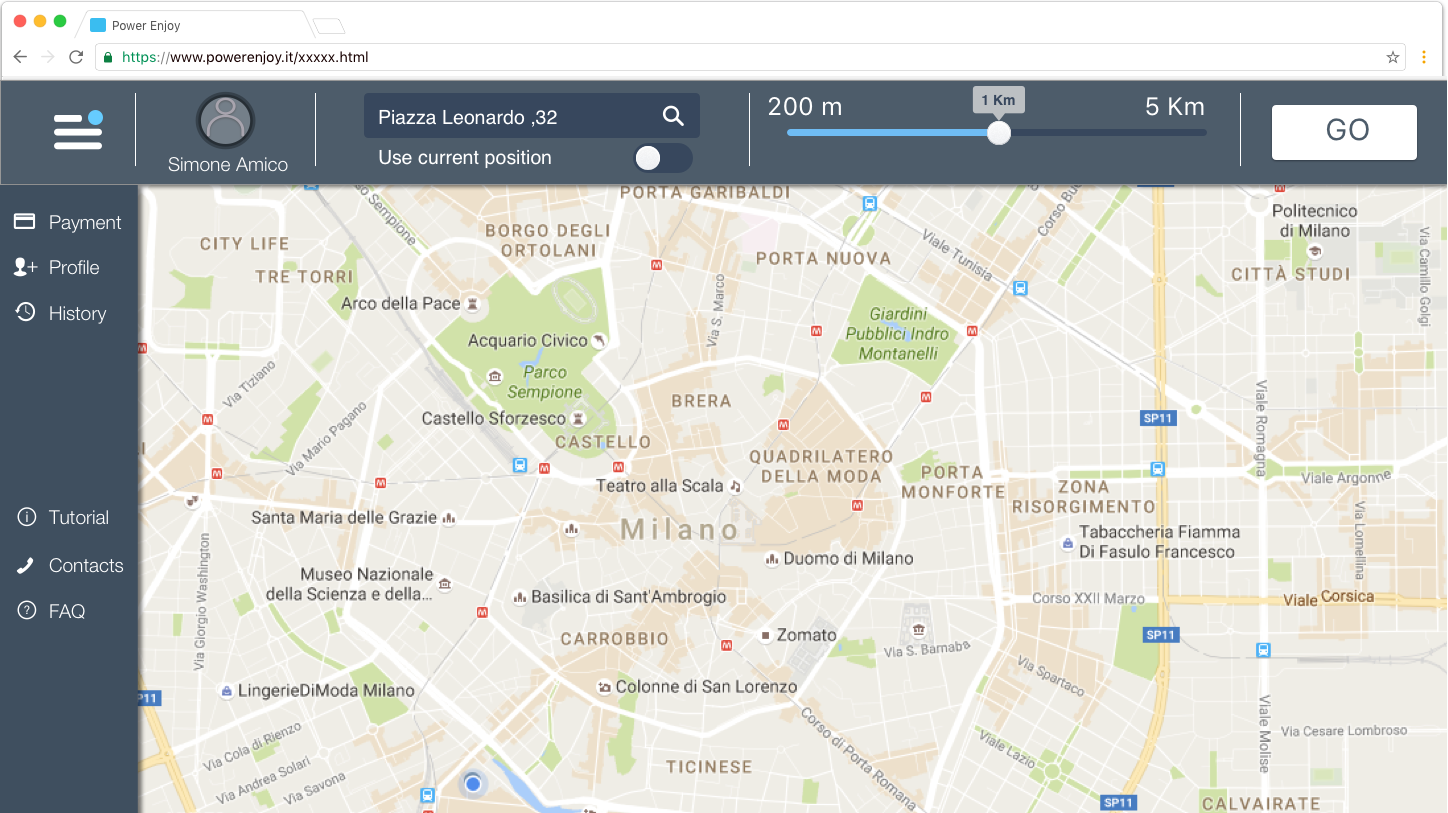
\includegraphics[scale=0.28]{Images/webApp/MainMenu.png}
		 \caption{Main page with account info bar}
		\end{figure}
		\clearpage
		
		
		%-------------------
		%	3.1.3 ONBOARD
		%-------------------
		
		\FloatBarrier
 	 	\subsubsection{On-Board Application (Touch)}
 	 	 \begin{figure}
		 \centering	
		\vspace{-17cm}		 
		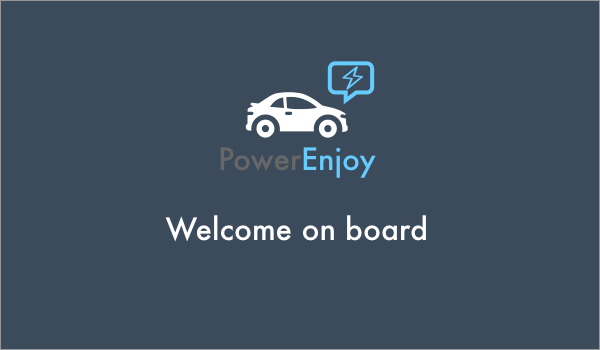
\includegraphics[scale=0.6]{Images/onBoard/Welcome.png}
		 \caption{Welcome screen}
		 \centering
 	 	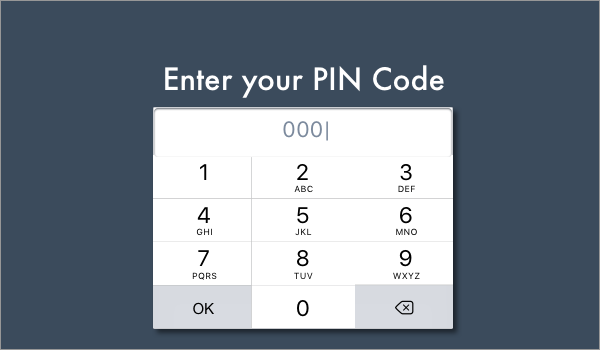
\includegraphics[scale=0.6]{Images/onBoard/Pin.png}
		  \caption{Pin request}
 	 	\end{figure}
 	 	\clearpage
 	 	\begin{figure}
		 \centering	
		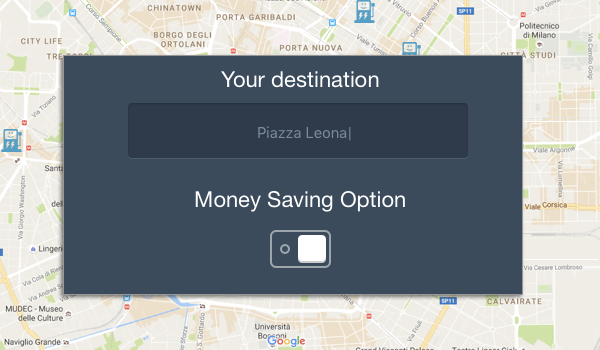
\includegraphics[scale=0.6]{Images/onBoard/Destination.png}
		 \caption{Destination input screen}
		\centering
 	 	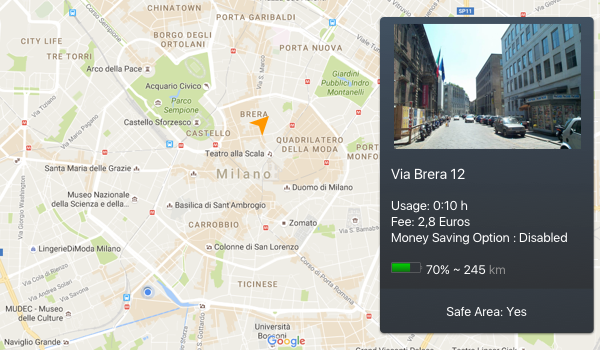
\includegraphics[scale=0.6]{Images/onBoard/Main.png}
		  \caption{Main screen}
 	 	\end{figure}
 	 	\clearpage
 	 	
 	 	
 	 	%------------------
 	 	% 3.2 SCENARIO
 	 	%------------------
 	 	\newpage
 	 	\subsection{Scenarios}
 	 	
 	 	\subsubsection{Scenario 1:User sign-up}
 	 	Maria is going out with friends for dinner .She doesn't own a 
 	 	car but has to travel to the other side of the city. She knows that a taxi ride  
 	 	would be expensive and other forms of public transport are packed with people during
 	 	rush hour. She decides to download the PowerEnjoy application. Once the download is 
 	 	completed she fill out the necessary registration informations providing a valid 
 	 	license and payment method and is ready to go and enjoy the evening with her friends.
 	 	\FloatBarrier
		\import{Tables/}{UseCase1.tex} 	 	
		\newpage
		\setcounter{figure}{0}    
		\begin{figure}[htbp]
		 \caption{User registration sequence diagram}
		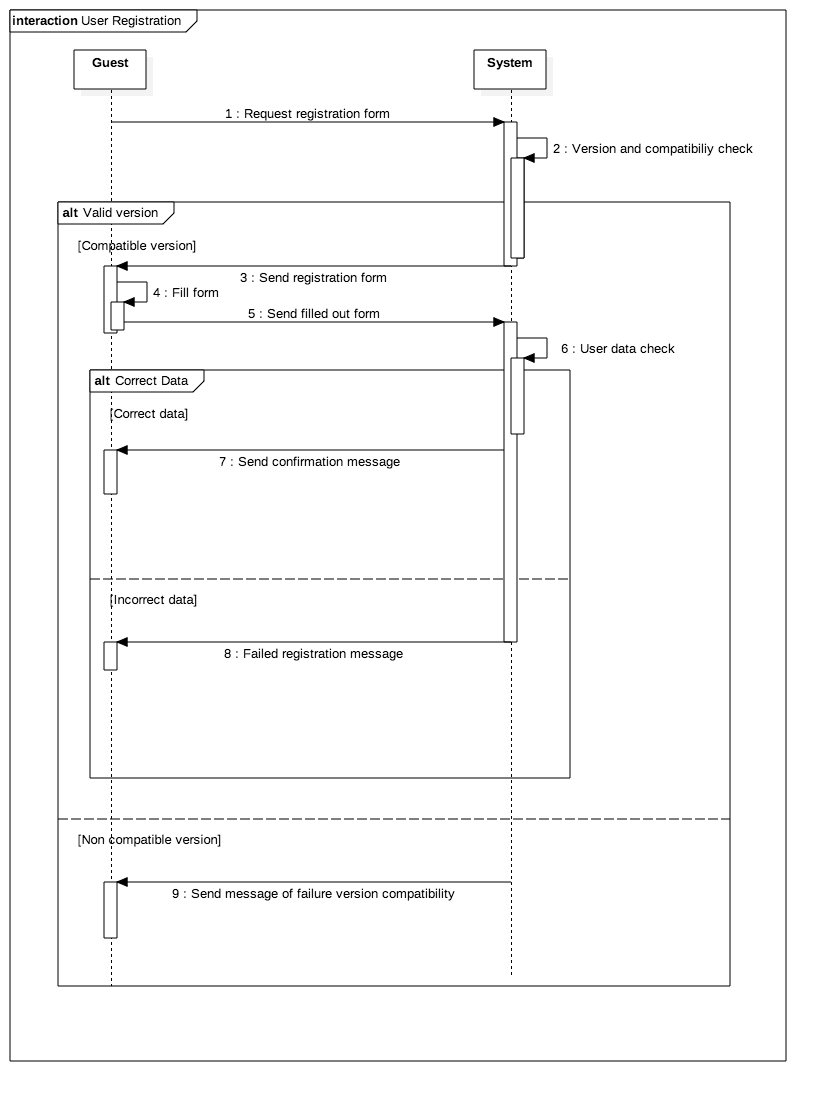
\includegraphics[scale=0.49]{Images/SequenceDiagram/UserRegistration.png}
 	 	\end{figure}
 	 	\clearpage
 	 	
		\subsubsection{Scenario 2: Log in}
		Angelo woke up late for his exam and has to hurry up. The bus stop is too far away 
		from his University so he has to find an alternative. So he logs into the system to
		look immediately for a car.
		
		\FloatBarrier
		\import{Tables/}{UseCase2.tex}
		\newpage
		\begin{figure}[htbp]
		 \caption{User login sequence diagram}
		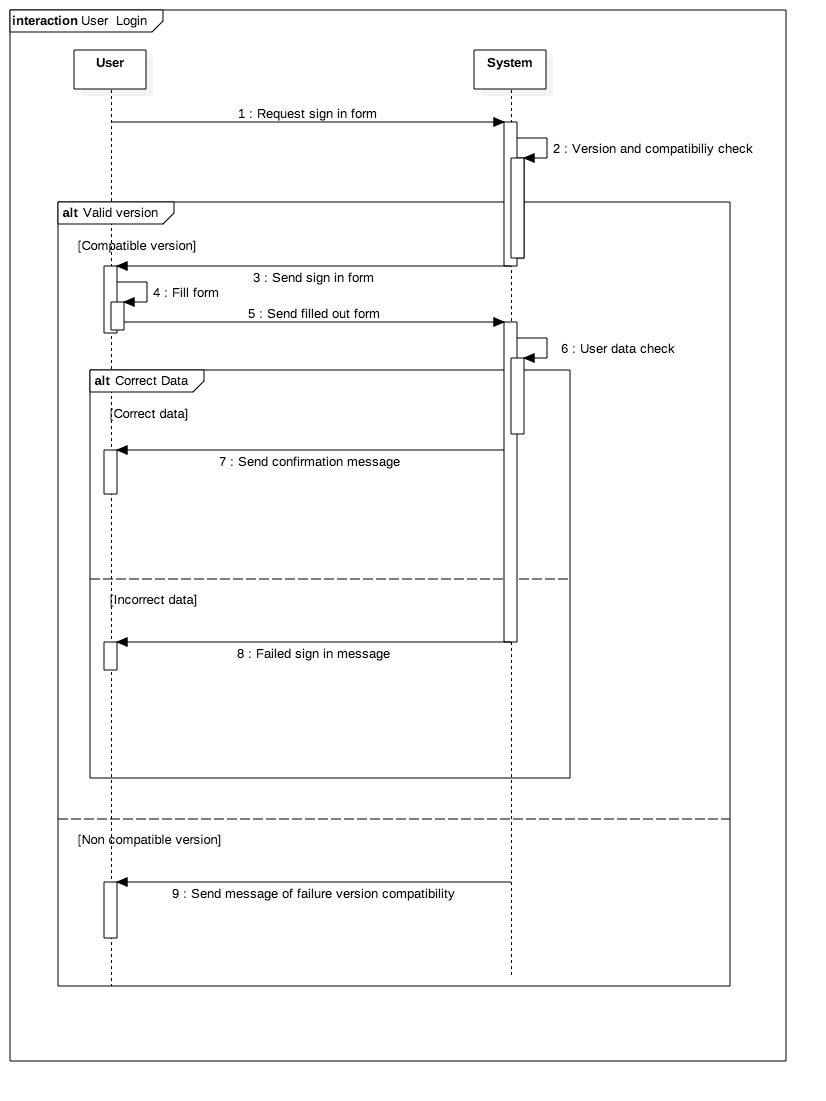
\includegraphics[scale=0.49]{Images/SequenceDiagram/UserLogin.png}
 	 	\end{figure}
 	 	\clearpage
		
		\subsubsection{Scenario 3: Reserve a car}
		Francesca has to take the train. The station is far away so she has to drive but she
		doesn't want to leave her car parked in an expensive car lot. She decides to search 
		and reserve the nearest PowerEnjoy.
		
		\FloatBarrier
		\import{Tables/}{UseCase3.tex}
		\newpage
		\begin{figure}[htbp]
		 \caption{Car reservation sequence diagram}
		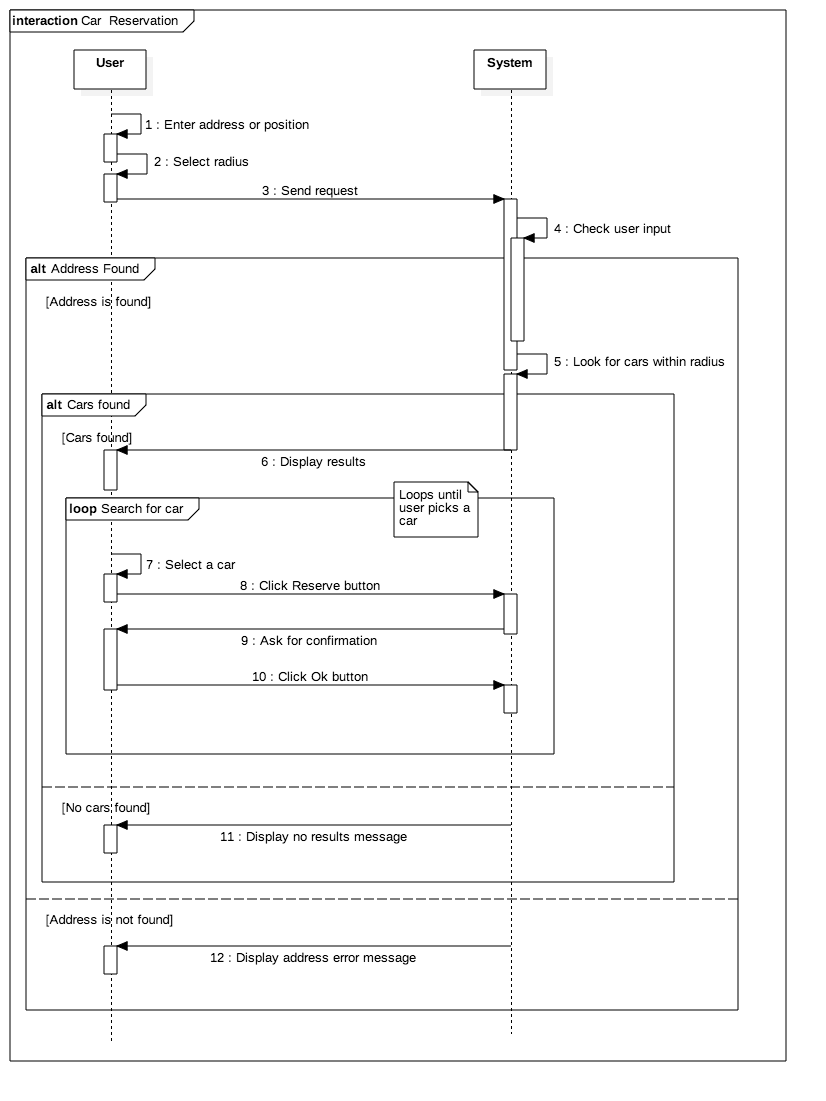
\includegraphics[scale=0.49]{Images/SequenceDiagram/CarReservation.png}
 	 	\end{figure}
 	 	\clearpage
		 
		\subsubsection{Scenario 4: Unable to reach car in time}
		Giacomo wants to meet his friends at the cinema. He reserves a car near him but as he 
		steps out of his front door he meets an old friend who offers him a lift.Giacomo
		never reaches the car he reserved so he has to pay a fee of 1 Euro for not unlocking
		the car within one hour.
		\FloatBarrier
		\import{Tables/}{UseCase4.tex}
		\newpage
		\begin{figure}[htbp]
		 \caption{Unable to reach car in time sequence diagram}
		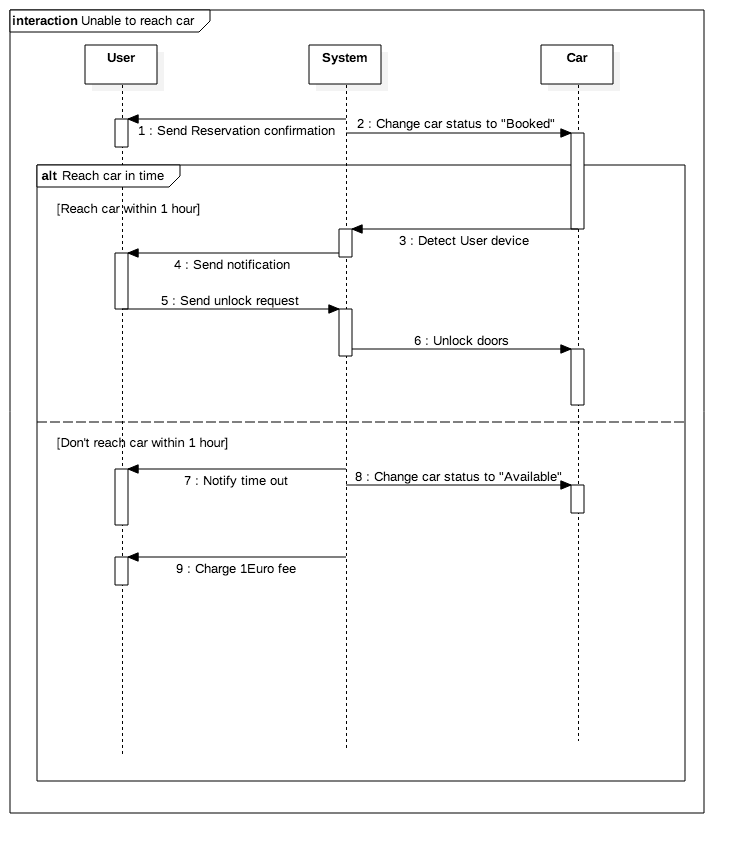
\includegraphics[scale=0.49]{Images/SequenceDiagram/Unable.png}
 	 	\end{figure}
 	 	\clearpage
		
		\subsubsection{Scenario 5: Report a problem}
		Gianni reserved a car but once he reached it he notices that the car has a flat
		tire. So he calls the Support Operator for help.
		\FloatBarrier
		\import{Tables/}{UseCase5.tex}
		\begin{figure}[htbp]
		 \caption{Report a problem}
		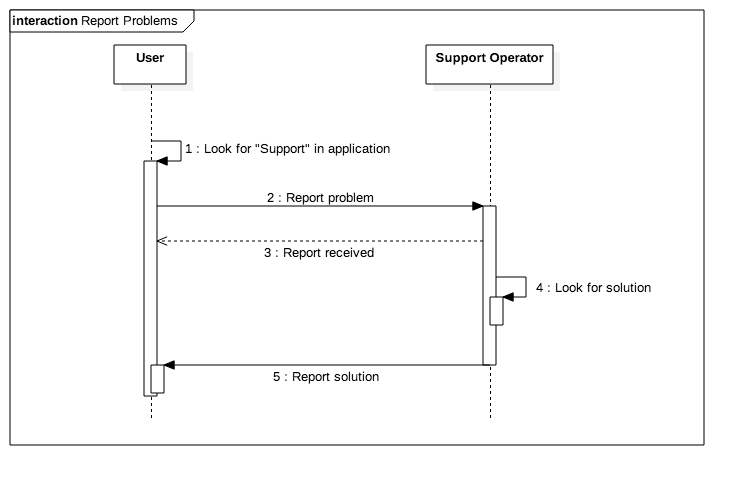
\includegraphics[scale=0.49]{Images/SequenceDiagram/Report.png}
 	 	\end{figure}
 	 	\clearpage
		
		\subsubsection{Scenario 6: Share ride with passengers}
		Lucia's parents are in town and she has to pick them up a the airport. She reserves
		a PowerEnjoy car as she knows that she will get a discount of 10\% on the ride's fee
		if she takes two passengers with her.
		\FloatBarrier
		\import{Tables/}{UseCase6.tex}
		\newpage
		\begin{figure}[htbp]
		 \caption{Shared ride sequence diagram}
		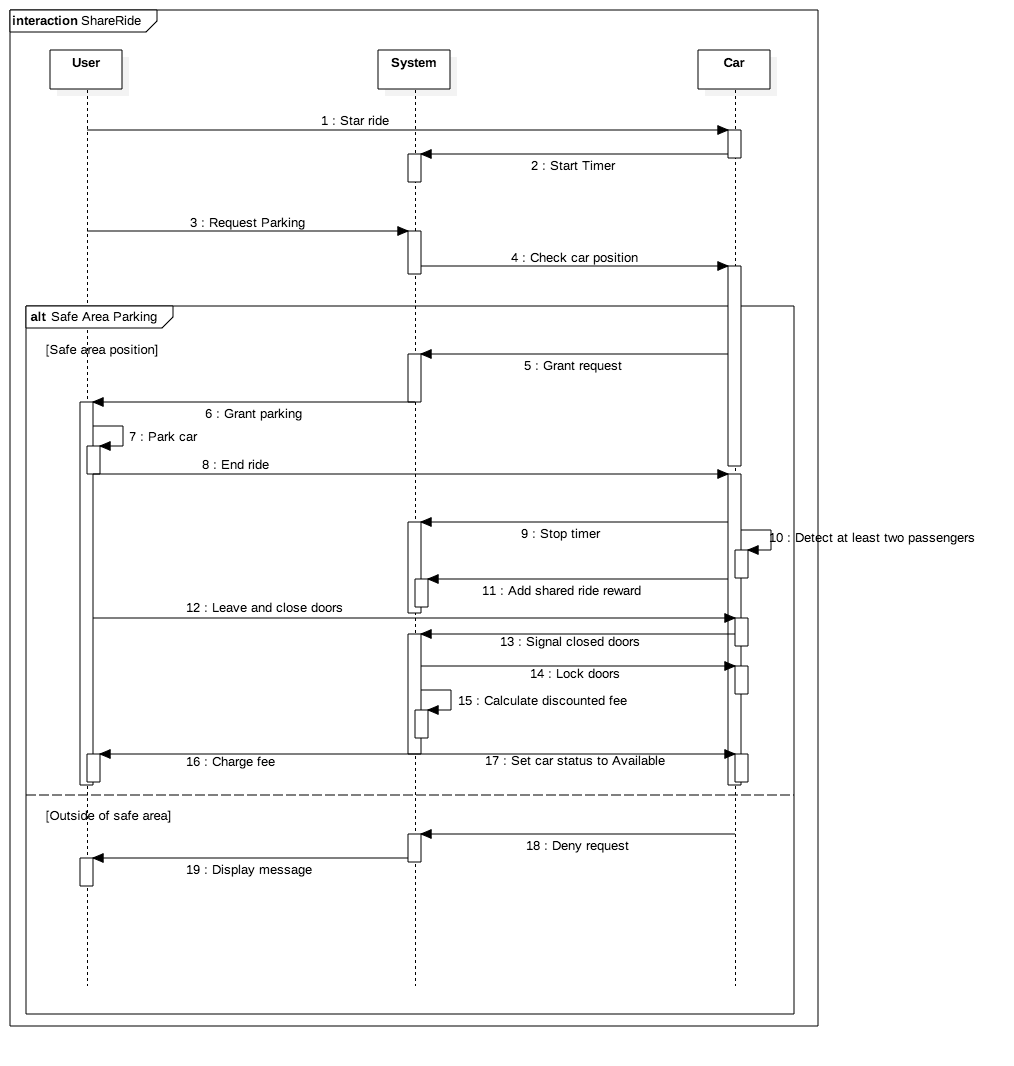
\includegraphics[scale=0.49]{Images/SequenceDiagram/ShareRide.png}
 	 	\end{figure}
 	 	\clearpage
		
		\subsubsection{Scenario 7: Drive with Money Saving Option}
		Flavio wants to attend his brother football match. He decides to use the money saving 
		option which automatically shows him the optimal parking solution closest to his destination.
		In return he gets a discount on his ride's fee.
		\FloatBarrier
		\import{Tables/}{UseCase7.tex}
		\newpage
		\begin{figure}[htbp]
		\caption{Money saving option sequence diagram}
		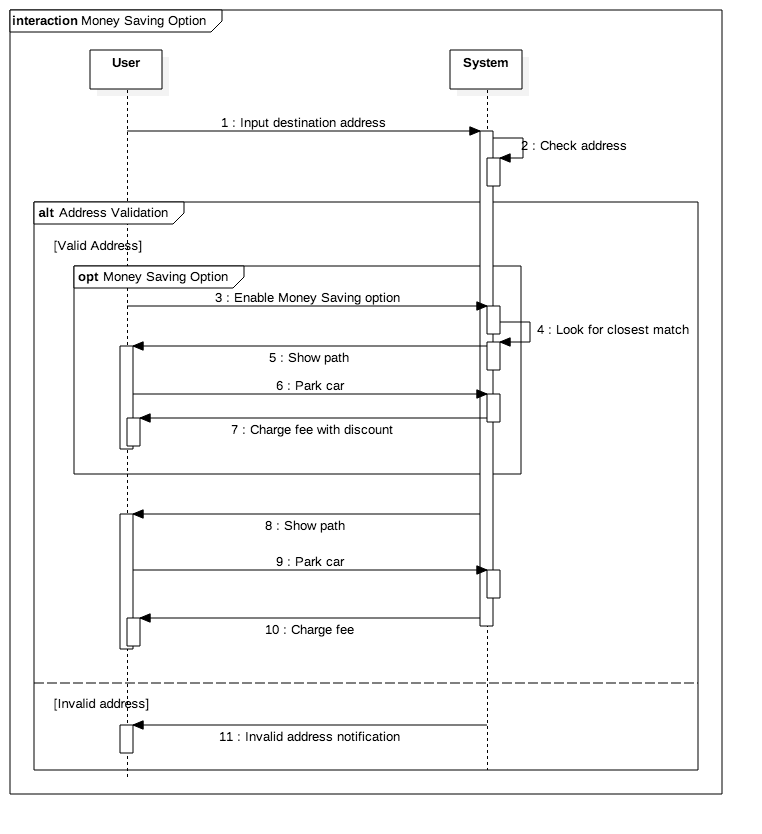
\includegraphics[scale=0.49]{Images/SequenceDiagram/MSO.png}
 	 	\end{figure}
 	 	\clearpage
		
		\subsubsection{Scenario 8: Leaving a car with battery level at \textgreater 50\%}
		After a long day working , Edoardo is tired but has to visit his ill mother who lives not too
		far away. He reserves a car and takes a short ride to his destination. He leaves the car with
		a battery level over 50\% so he's entitled to get a discount of 20\% on his fee.
		\FloatBarrier
		\import{Tables/}{UseCase8.tex}
		\newpage
		\begin{figure}[htbp]
		\caption{Park car with battery level \textgreater 50\% sequence diagram}
		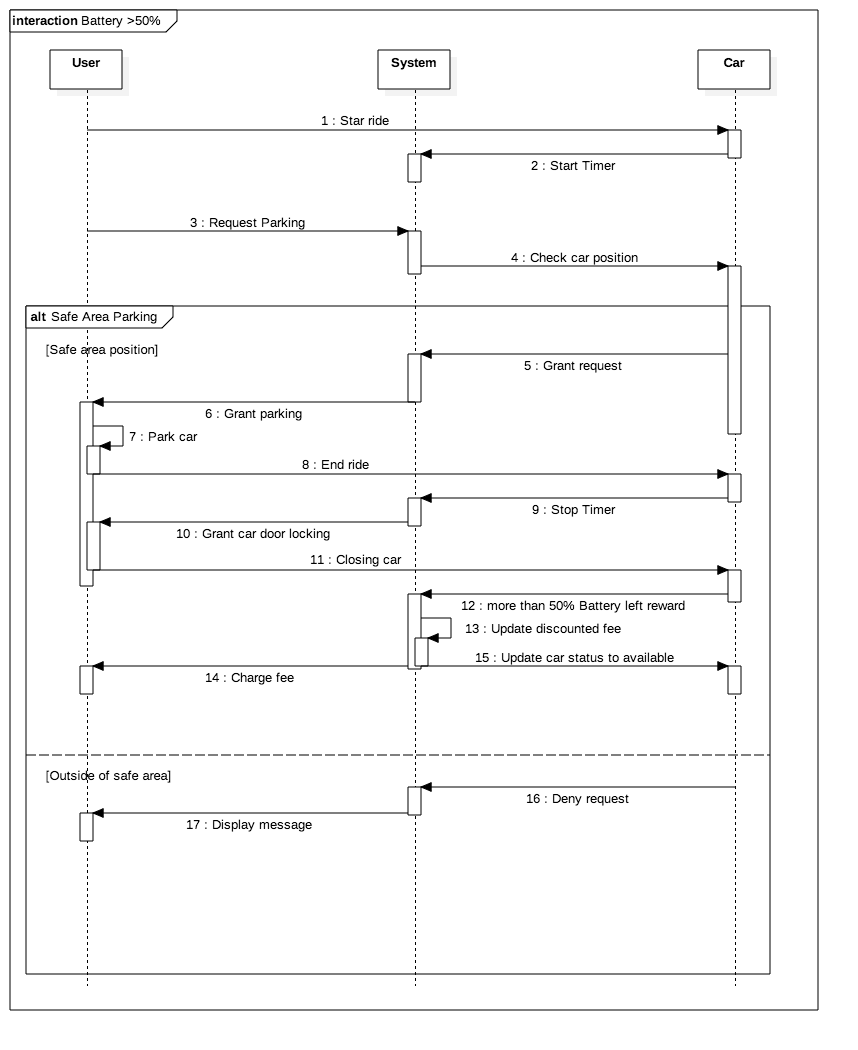
\includegraphics[scale=0.49]{Images/SequenceDiagram/Battery.png}
 	 	\end{figure}
 	 	\clearpage
		
		\subsubsection{Scenario 9: Charge car}
		Daniele is driving a PowerEnjoy car to get to the football stadium. Near the stadium there is a 
		PowerEnjoy charging station. He decides to park the car there and to plug it into the 
		charging station : as a reward PowerEnjoy applies a discount of 30\% on his fee.
		\FloatBarrier
		\import{Tables/}{UseCase9.tex}
		\newpage
		\begin{figure}[htbp]
		\caption{Car charging sequence diagram}
		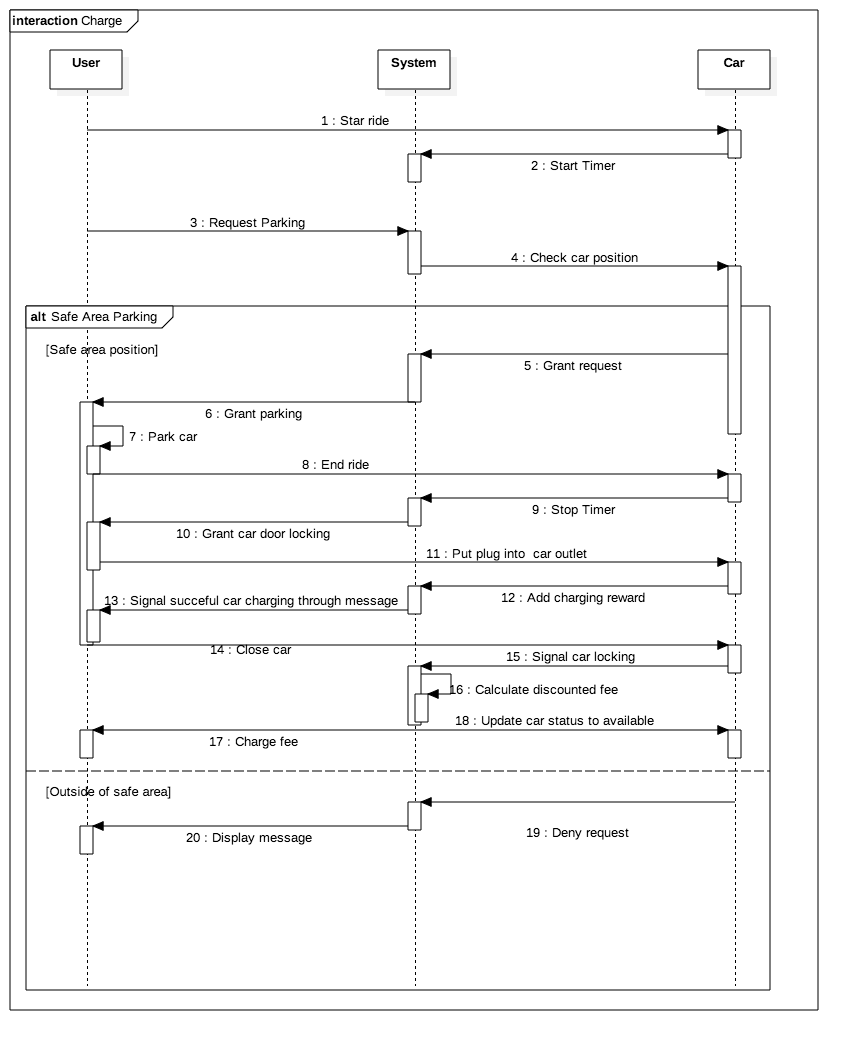
\includegraphics[scale=0.49]{Images/SequenceDiagram/Charge.png}
 	 	\end{figure}
 	 	\clearpage
		
		
		\subsubsection{Scenario 10: Out of safe area parking}
		Andrea has to meet his girlfriend's parents in the suburbs. He decides to take a PowerEnjoy
		and park on a private driveway. Unfortunately the parking spot is marked as \emph{unsafe} so 	
		the onboard  display notifies him about the situation. This way Andrea parks the car in an
		accessible position for everyone.
		\FloatBarrier
		\import{Tables/}{UseCase10.tex}
		\newpage
		\begin{figure}[htbp]
		\caption{Out of safe area parking sequence diagram}
		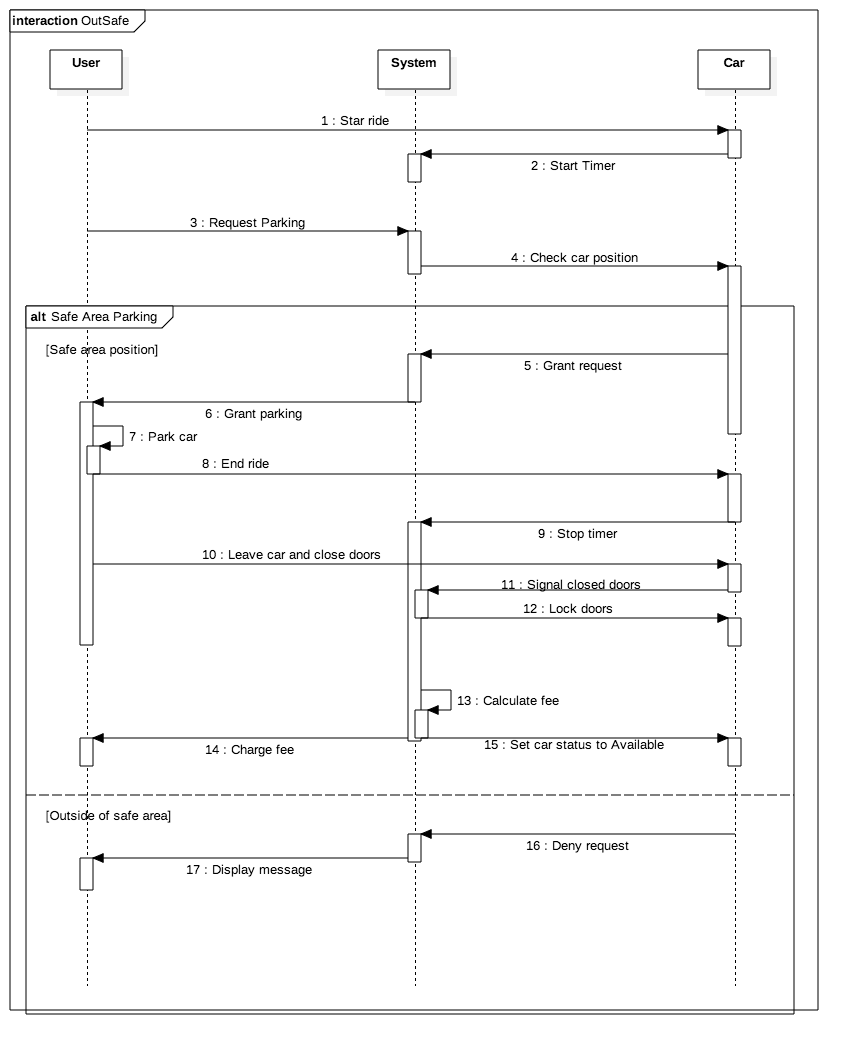
\includegraphics[scale=0.49]{Images/SequenceDiagram/OutSafe.png}
 	 	\end{figure}
 	 	\clearpage
		
		\subsubsection{Scenario 11: Additional fee charged}
		Alessandro is running late for his date and decides the park his reserved car as close as 
		possible. Unfortunately he parks the car far away from the nearest power grid : PowerEnjoy 
		has to take care of this situation , so Alessandro is charged with an additional 30\% on his
		ride's fee.
		\FloatBarrier
		\import{Tables/}{UseCase11.tex}
		\newpage
		\begin{figure}[htbp]
		\caption{Parking with additional fee sequence diagram}
		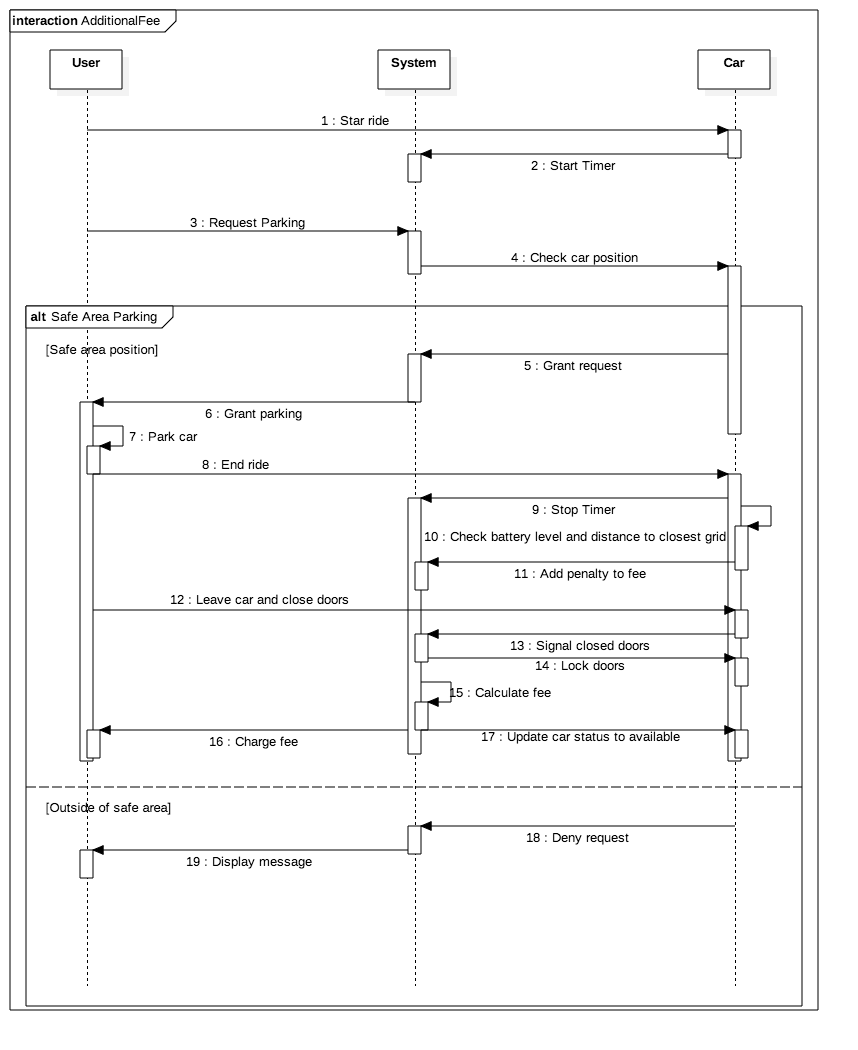
\includegraphics[scale=0.49]{Images/SequenceDiagram/AdditionalFee.png}
 	 	\end{figure}
 	 	\clearpage
 	 	
		\subsubsection{Scenario 12: User information update}
		Leonardo's credit card is expiring next week. As PowerEnjoy requires a valid payment method ,
		Leonardo decides to update his payment method.
		\FloatBarrier
		\import{Tables/}{UseCase12.tex}
		\newpage
		\begin{figure}[htbp]
		\begin{center}
		\caption{Modify user data sequence diagram}
		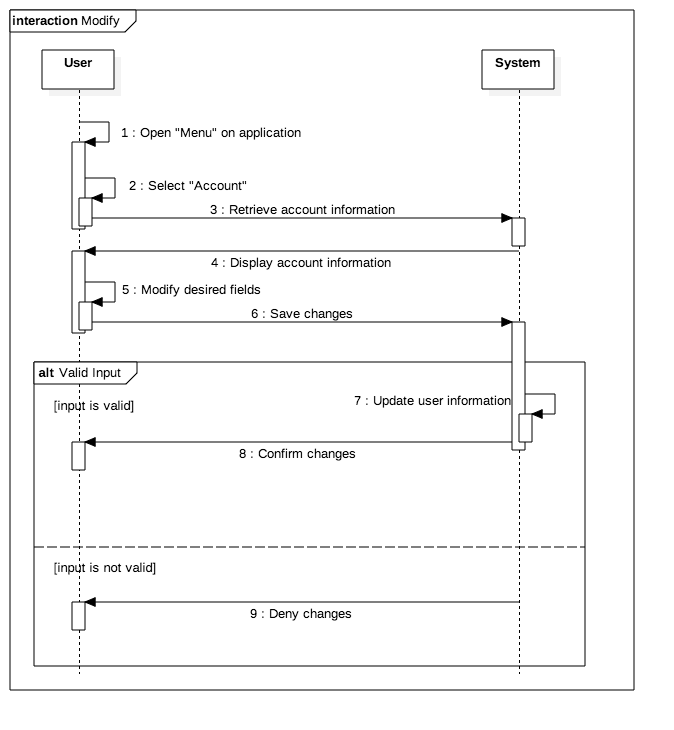
\includegraphics[scale=0.51]{Images/SequenceDiagram/Modify.png}
		\end{center} 	 	
 	 	\end{figure}
 	 	\clearpage
 	 	
 	 	
 	 	%--------------------
 	 	% CLASS DIAGRAM
 	 	%--------------------
 	 	 \FloatBarrier
 	 	\subsection{Class Diagram}
 	 	This class diagram gives an general and not detailed overview on how the system is intended to be implemented. Extensibility is an important facotr as future growth must be taken in account.
 	 	\begin{figure}
		\vspace{-16cm}		
		\begin{center}
		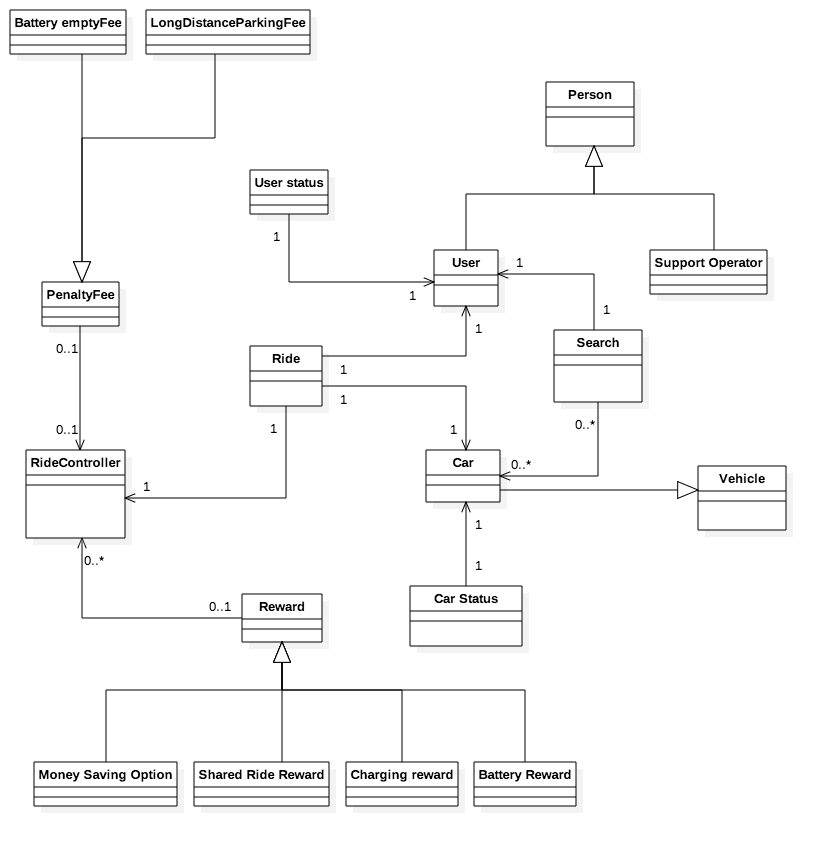
\includegraphics[scale=0.49]{Images/ClassDiagram/General.png}
		\end{center} 	 	
 	 	\end{figure}
 	 	\clearpage
 	 	\newpage
 	 	%--------------------
 	 	% STATE CHARTS 
 	 	%--------------------
 	 	
 	 	\subsection{State charts}
 	 	This section shows the user action event flow and the car ride event flow with the help of 
 	 	two state charts.
		\FloatBarrier
  		\begin{figure}[htbp]
		\centering	
		 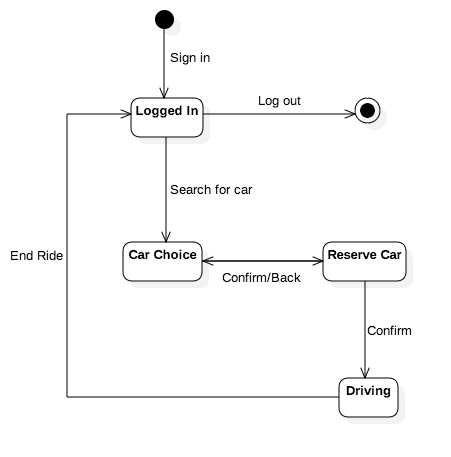
\includegraphics[scale=0.6]{Images/StateChart/Login.png}
		 \caption{User state chart}
		 \end{figure}
		 \begin{figure}
		 \centering
 	 	  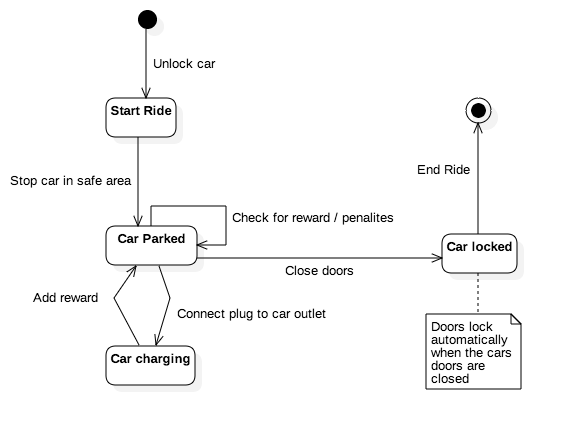
\includegraphics[scale=0.6]{Images/StateChart/Bonus.png}
 	 	  \caption{Ride state chart}
 	 	\end{figure}
 	 	\clearpage
 	 	\newpage
 	 \subsection{Alloy}
 	 \FloatBarrier
 	 \lstinputlisting[language=alloy]{PowerEnjoy.als}
 	 \newpage
	\begin{landscape} 	 
 	 \FloatBarrier 
 	 \begin{figure}
 	 \centering
 	 	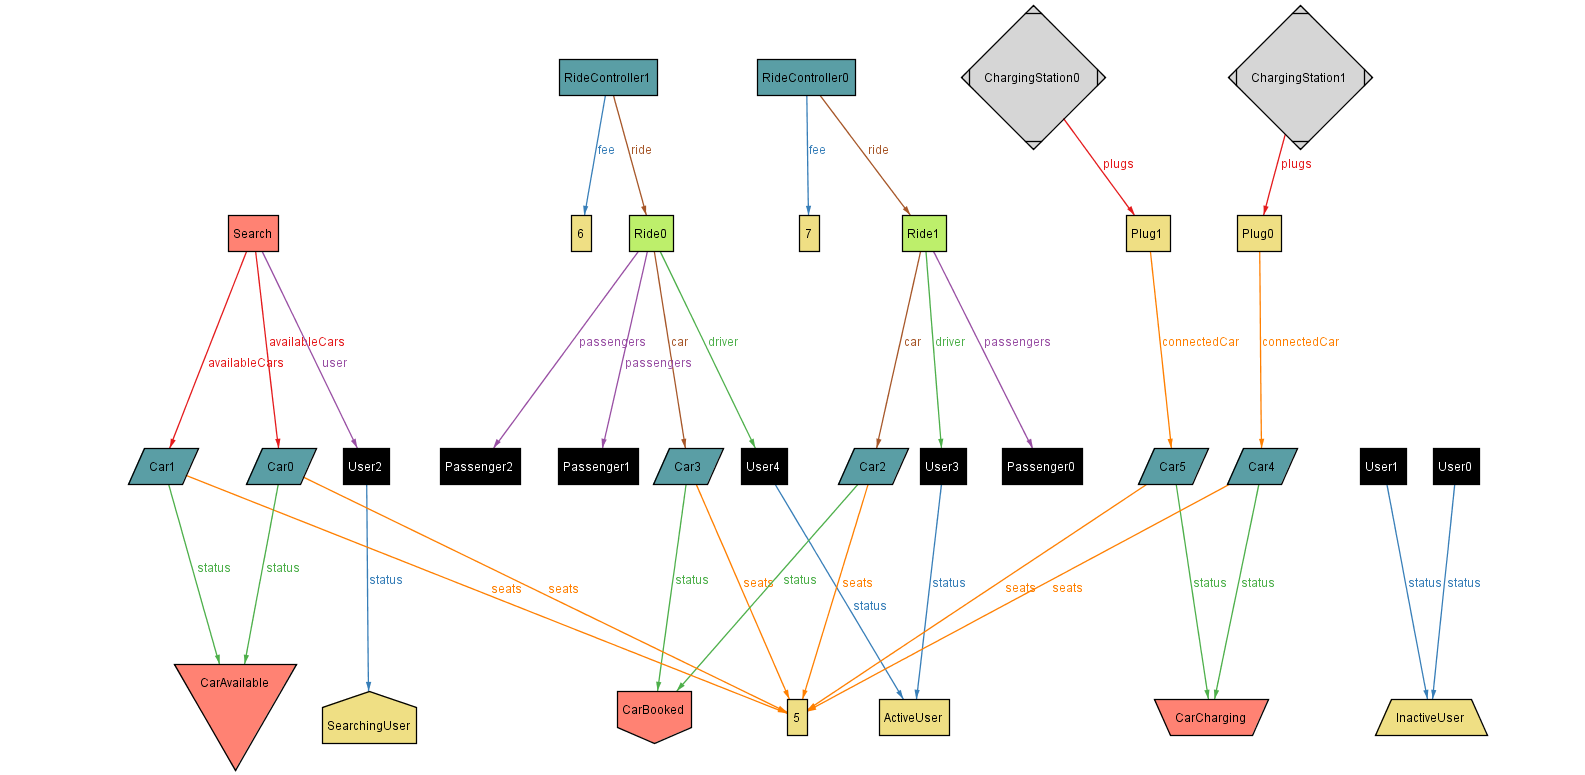
\includegraphics[scale=0.45]{Images/ALLOY1.png}
 	 \end{figure}
 	 \end{landscape}
 	 \newpage
 	 The alloy model simulates a common scenario : some user's are involved in rides which means that they 
 	 are drivers of a car that has to be booked. Some other user is doing a search which lists only 	
 	 available cars. A user doing in a search can't be inactive nor active (driving). Every ride has an associated fee . We chose to implement a Money Saving Option discount as example of the different discounts that can gained by users. Finally some cars are located in charging station , which are composed of plugs. Obviously a car can only be connected to only one plug at the time and if in a charging station it must be in 'charging' status.
		
\end{document}
